%Fixes pandoc tightlist error
\providecommand{\tightlist}{%
  \setlength{\itemsep}{0pt}\setlength{\parskip}{0pt}}

\documentclass[12pt]{article}
%\renewcommand{\familydefault}{\sfdefault}
\usepackage{amsfonts}
\usepackage{amssymb}
\usepackage{multicol}
\usepackage{graphicx}
\usepackage{subfig}
\usepackage{pdfpages}

\usepackage{titlesec}
\usepackage{longtable}
\usepackage{supertabular}

\usepackage{booktabs}
\setlength{\parindent}{0pt}
\setlength{\parskip}{1em}

\usepackage{hyperref}
\usepackage{pdflscape}

% Contents of listings-setup.tex
\usepackage{framed, xcolor}
\usepackage{listings}
\usepackage{framed}

\lstset{
    basicstyle=\ttfamily,
    numbers=left,
    keywordstyle=\color[rgb]{0.13,0.29,0.53}\bfseries,
    stringstyle=\color[rgb]{0.31,0.60,0.02},
    commentstyle=\color[rgb]{0.56,0.35,0.01}\itshape,
    numberstyle=\footnotesize,
    stepnumber=1,
    numbersep=5pt,
    backgroundcolor=\color[RGB]{248,248,248},
    showspaces=false,
    showstringspaces=false,
    showtabs=false,
    tabsize=2,
    captionpos=b,
    breaklines=true,
    breakatwhitespace=true,
    breakautoindent=true,
    escapeinside={\%*}{*)},
    linewidth=\textwidth,
    basewidth=0.5em,
}

%References

\usepackage[
backend=bibtex,
style=numeric,
autocite=footnote,
citestyle=authoryear
]{biblatex}

\addbibresource{references.bib}



\usepackage[british]{babel}
\usepackage{csquotes}

\usepackage{url}

\usepackage{microtype}

\usepackage{float}

\begin{document}

\section{Read Me}

The following documentation provides instructions on how to install and
use the application.

\subsection{Installation}\label{installation}

To install an Android application not available from the play store,
there are several steps that are required to install the app.

\subsubsection{Enable Unknown Sources}\label{enable-unknown-sources}

To install the application to a physical device it is necessary to
enable the setting to allow for installation of apps from unknown
sources; this is required as the application is not available from the
play store. The setting to allow unknown sources can be found in:
Settings \(\rightarrow\) Security \(\rightarrow\) Unknown sources:

\begin{figure}[H]
  \centering
  \subfloat[Security and Fingerprint]{{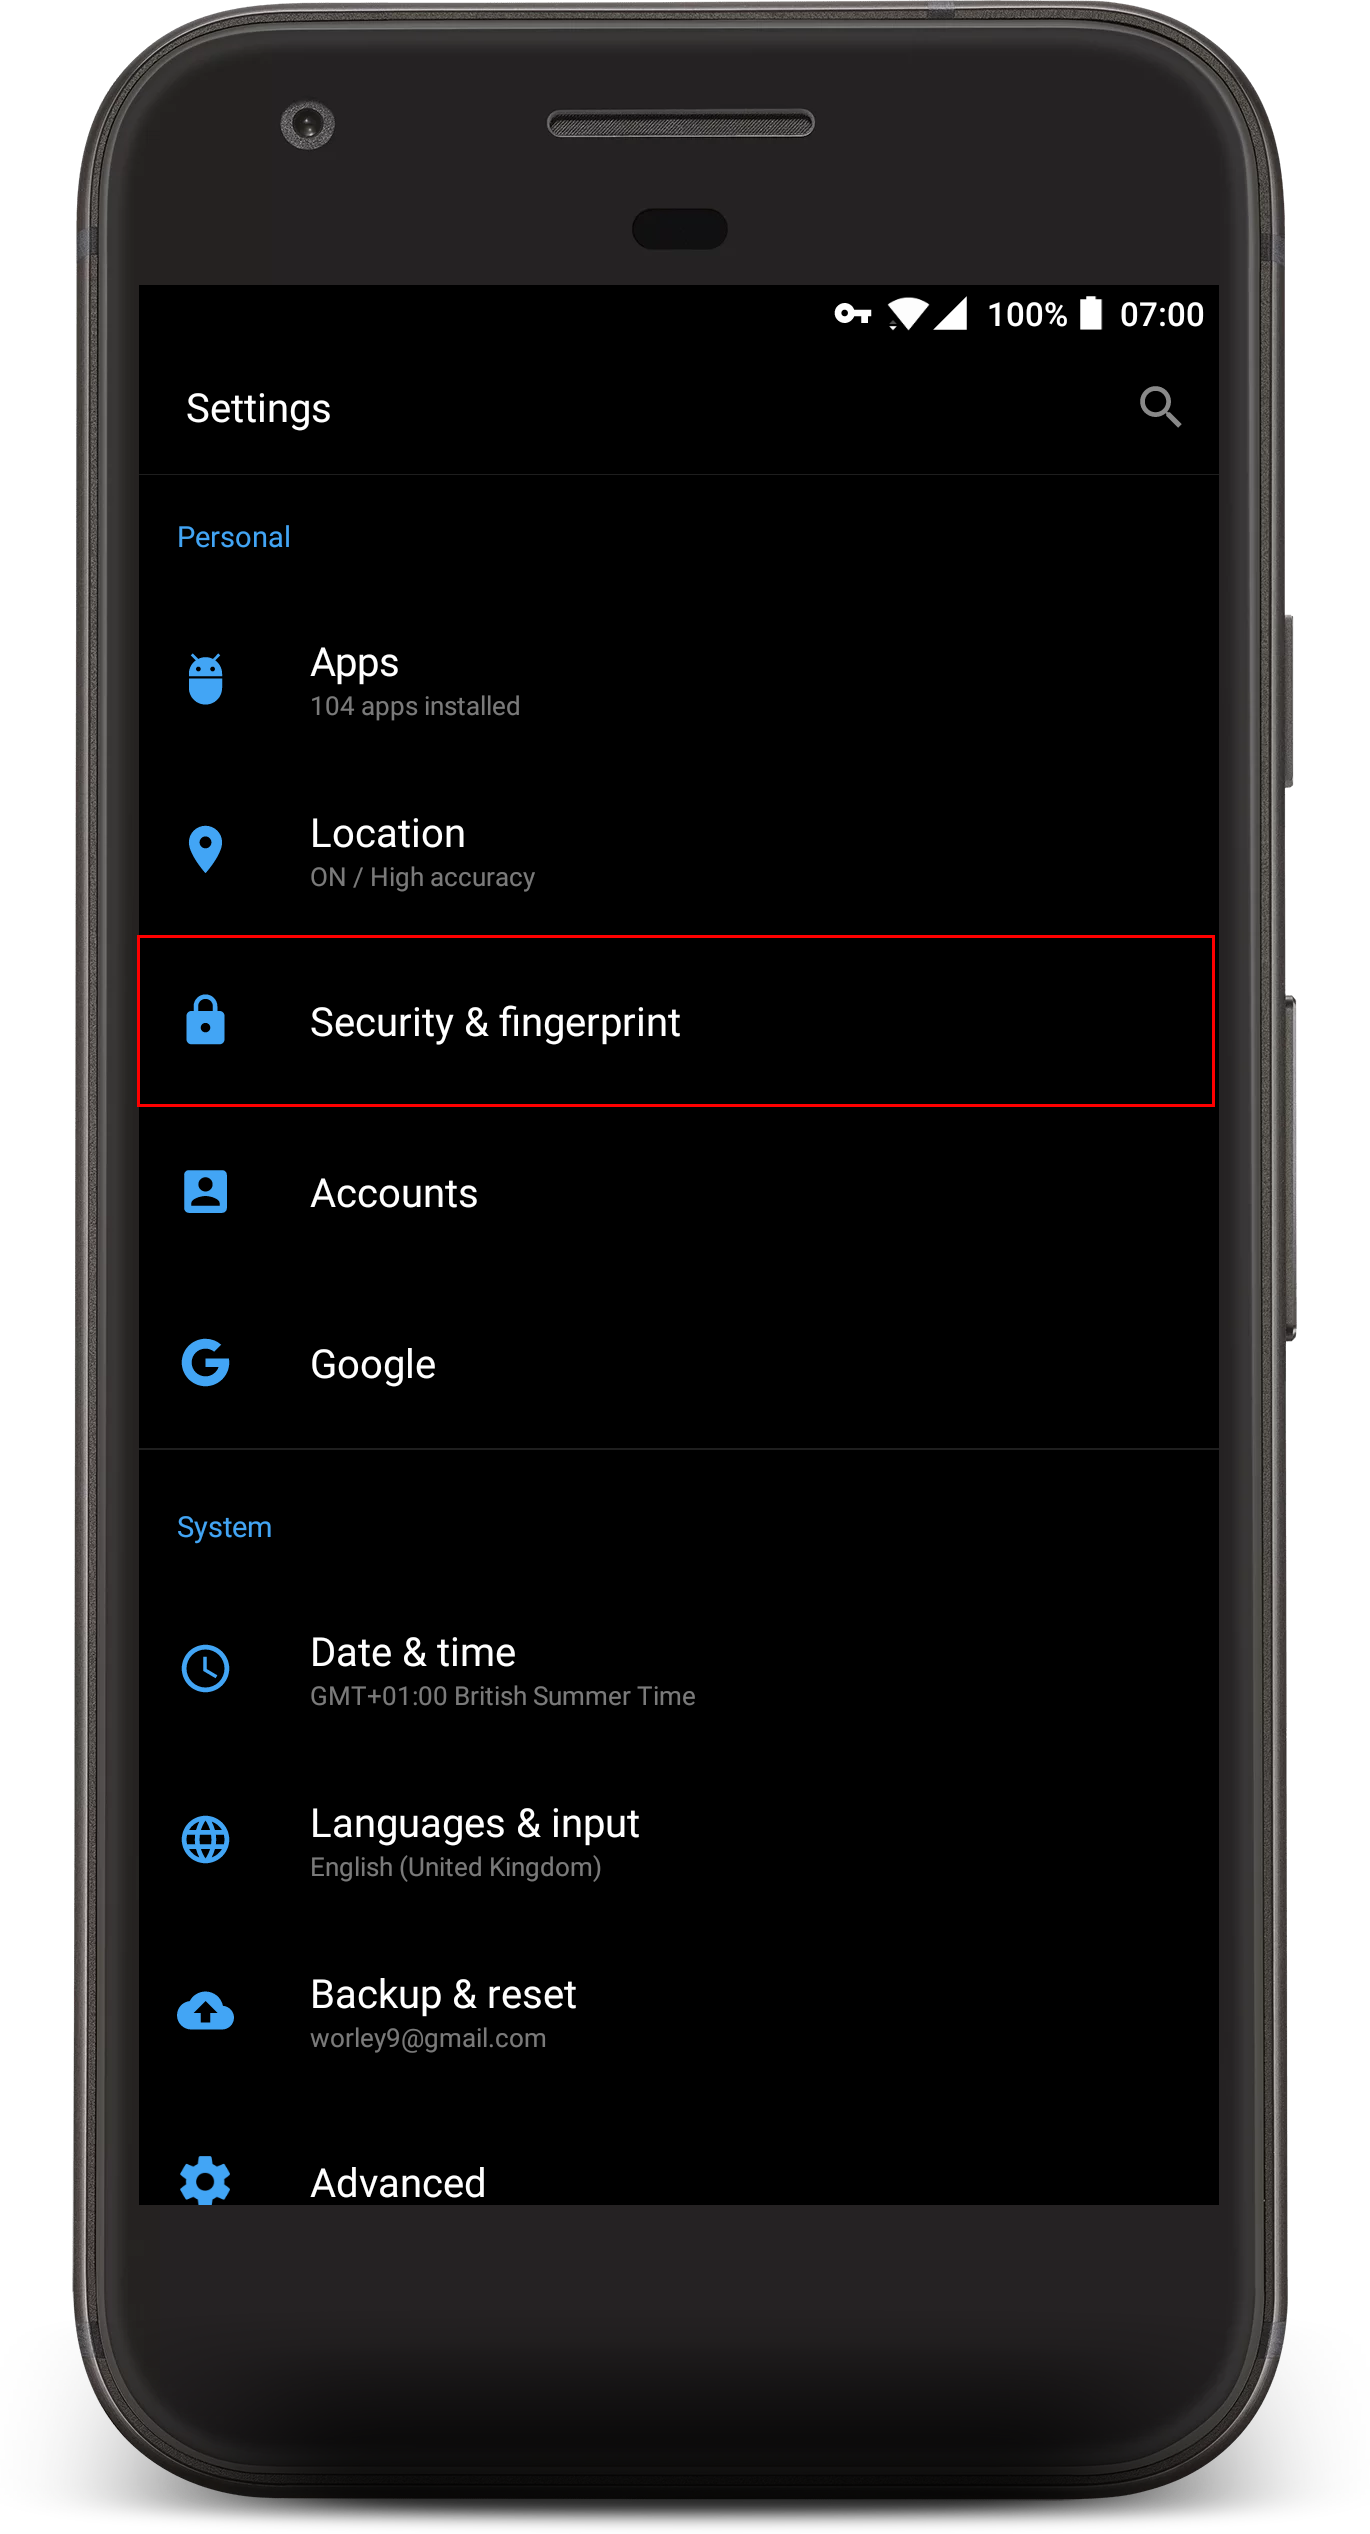
\includegraphics[scale=0.1]{./Images/security.png}}}
  \qquad
  \subfloat[Unknown sources enabled]{{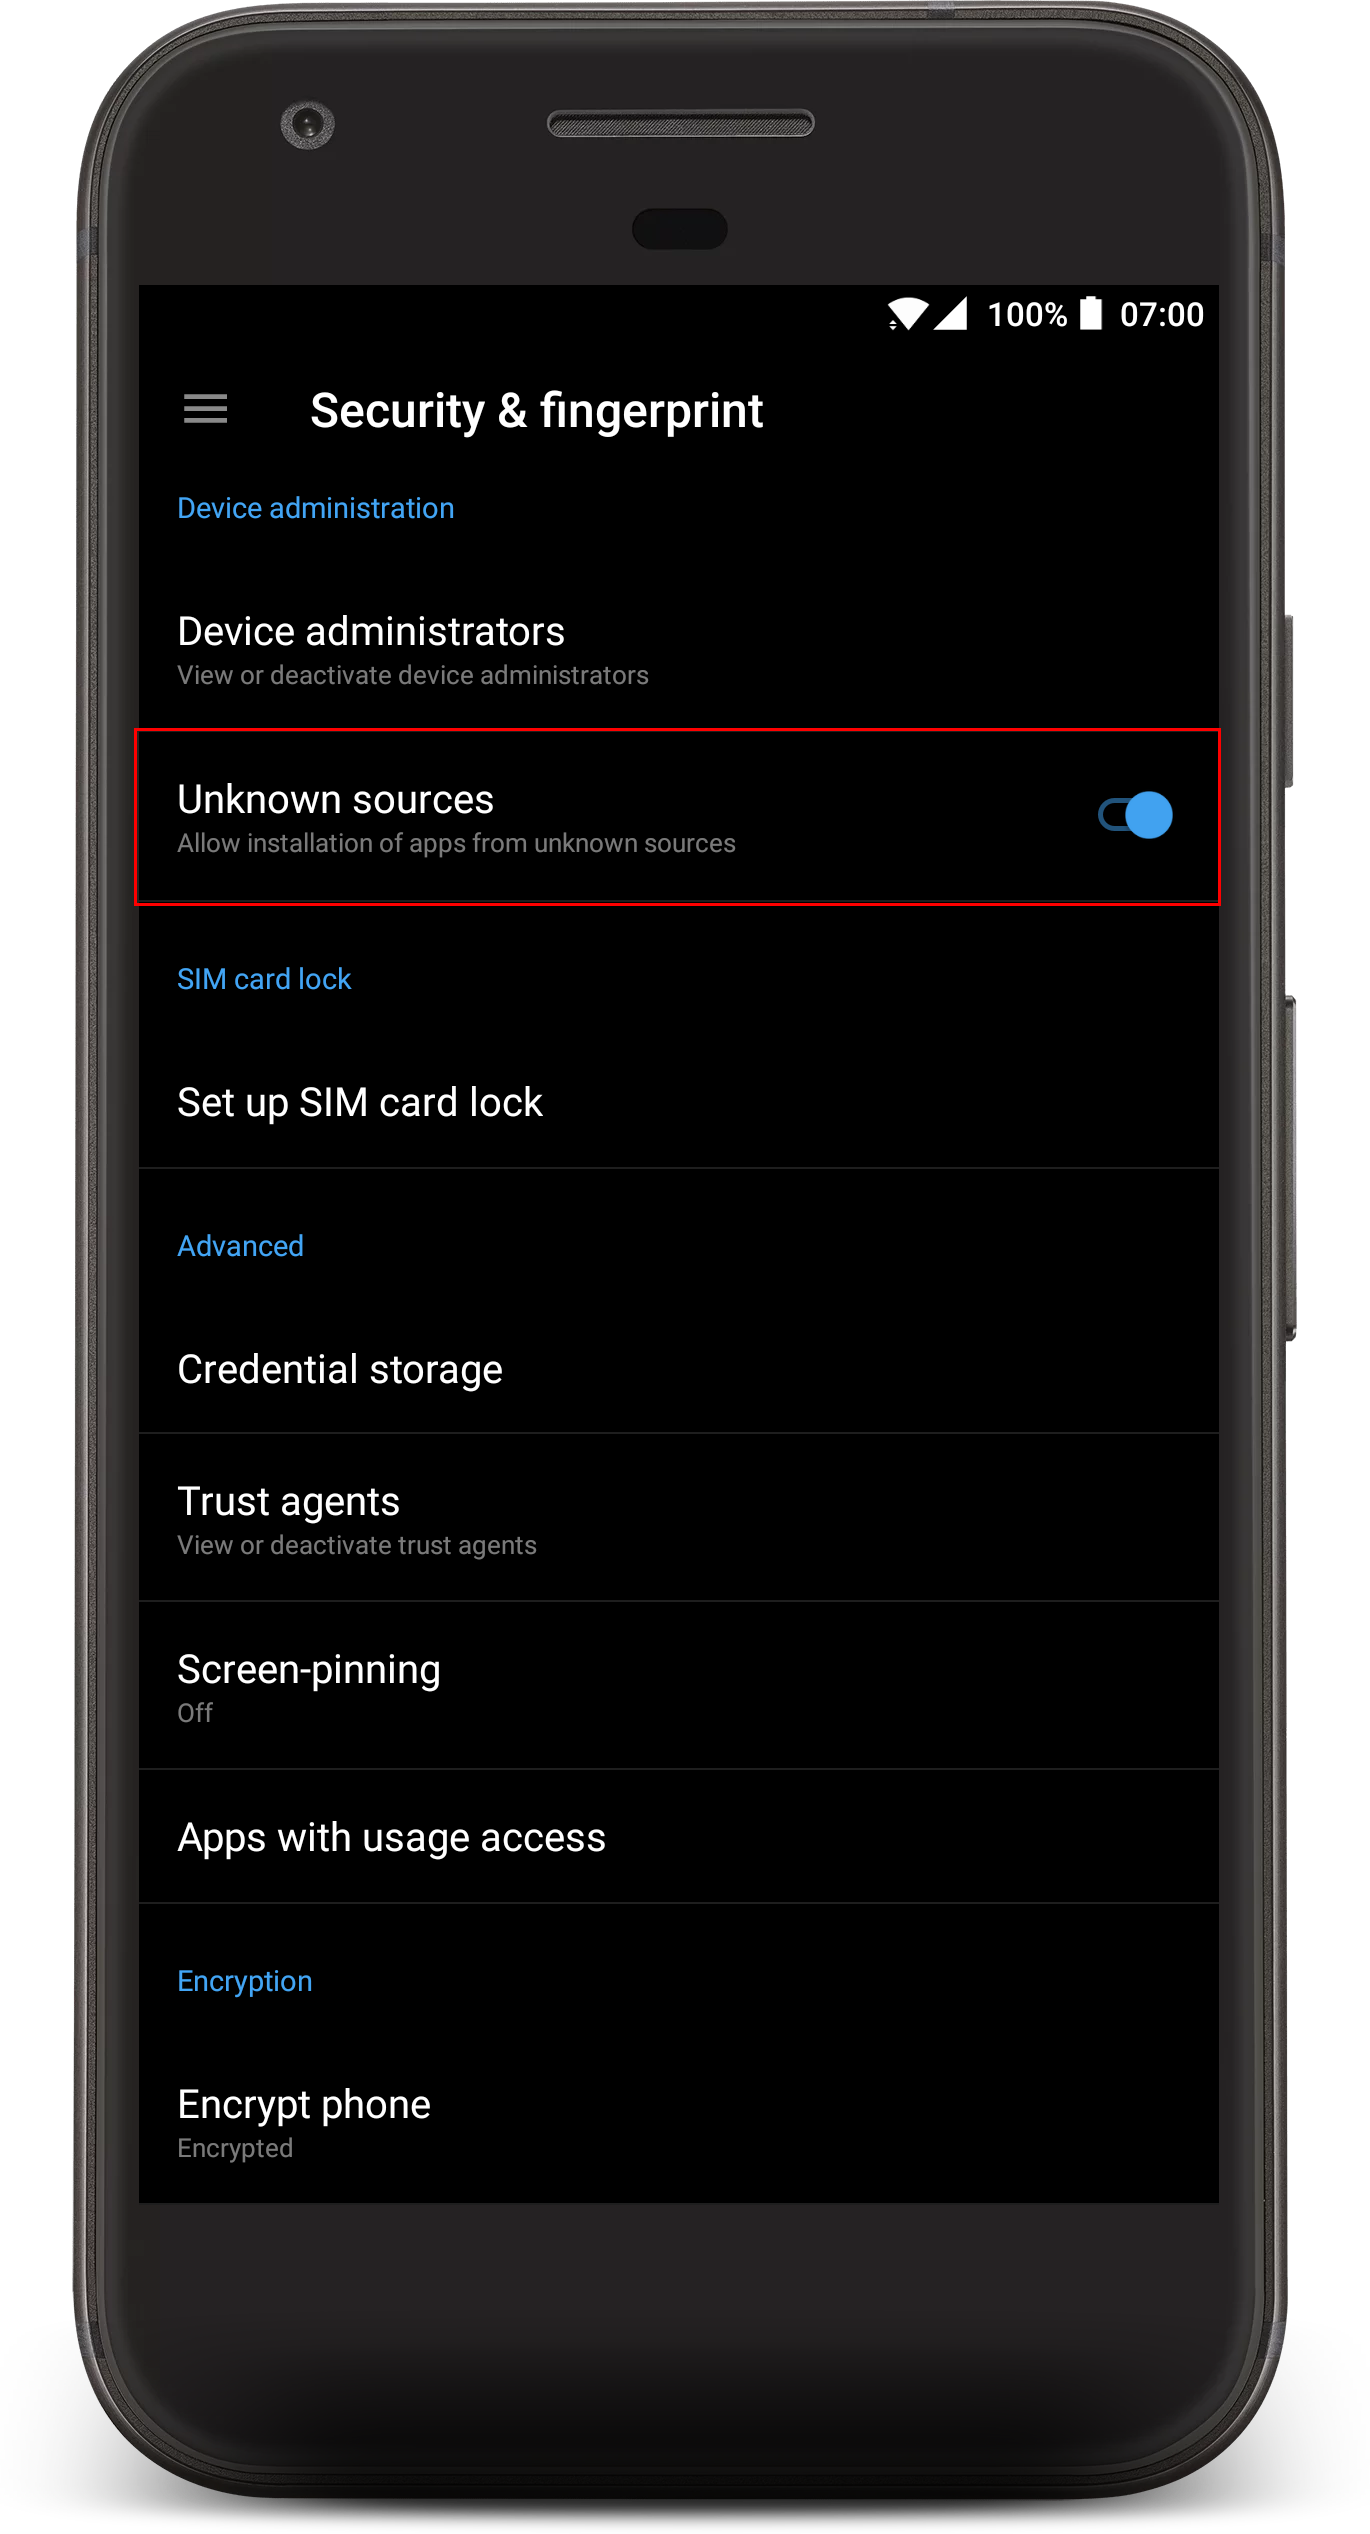
\includegraphics[scale=0.1]{./Images/unknownsources.png}}}

  \caption{Enabling unknown sources}%

  \label{fig:unknownsources}
\end{figure}

\subsubsection{Copy APK to Device and install
locally}\label{copy-apk-to-device-and-install-locally}

Once installation from unknown sources has been enabled, copy the
application APK to the device. On the device navigate to the location
that APK was copied to within the file browser on the device. Tap on the
APK and an installation prompt will be presented; accept the
installation and wait for the app to be installed.

When installation has been completed the app will now be available from
within the application draw or on the home-screen.

\subsubsection{Alternative Installation}\label{alternative-installation}

It is possible to install the application using the command line; in
this example it shows doing so using Windows 10 and the command line.

Before being able to install the application it is not only necessary to
enable unknown sources as above, but also to enable ADB debugging.

\subsubsection{Enable ADB on Device (Alternative
Installation)}\label{enable-adb-on-device-alternative-installation}

Enabling ADB can be done by first enabling developer options, go to
Settings \(\rightarrow\) About phone. From here you will need to tap the
\emph{Build number} around 7 times in succession, after which a success
message will show you have enabled developer settings.

\begin{figure}[H]
  \centering
  \subfloat[Enabling developer options]{{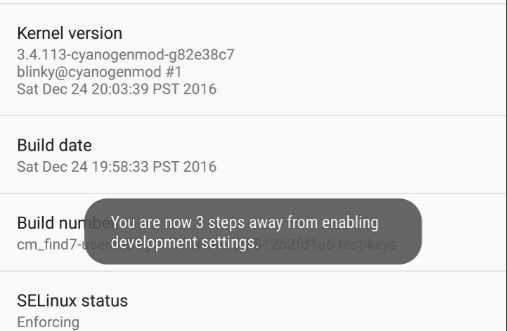
\includegraphics[scale=0.6]{./Images/enablingDeveloper.png}}}
  \qquad
  \subfloat[Developer options enabled message \label{fig:developerAvailable}]{{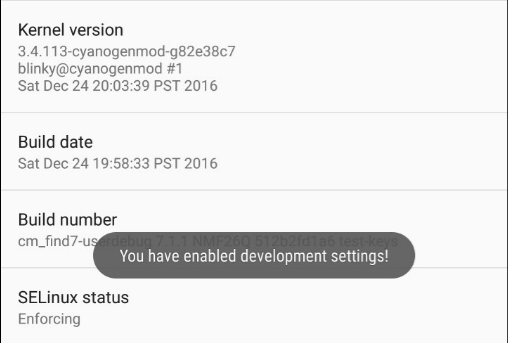
\includegraphics[scale=0.6]{./Images/developerSuccess.png}}}
  \caption{Enabling developer options}
  \label{fig:enablingDeveloperoptions}
\end{figure}

Developer settings are now available from within the settings menu as
shown in figure \ref{fig:developerOption}. Enter this option and scroll
to the option \emph{Android debugging} as shown in figure
\ref{fig:adbOption}, when toggled a warning message will appear (figure
\ref{fig:enableAdbMsg}); read and accept the warning to enable ADB.

\begin{figure}[H]
  \centering
  \subfloat[Developer option is now available \label{fig:developerOption}]{{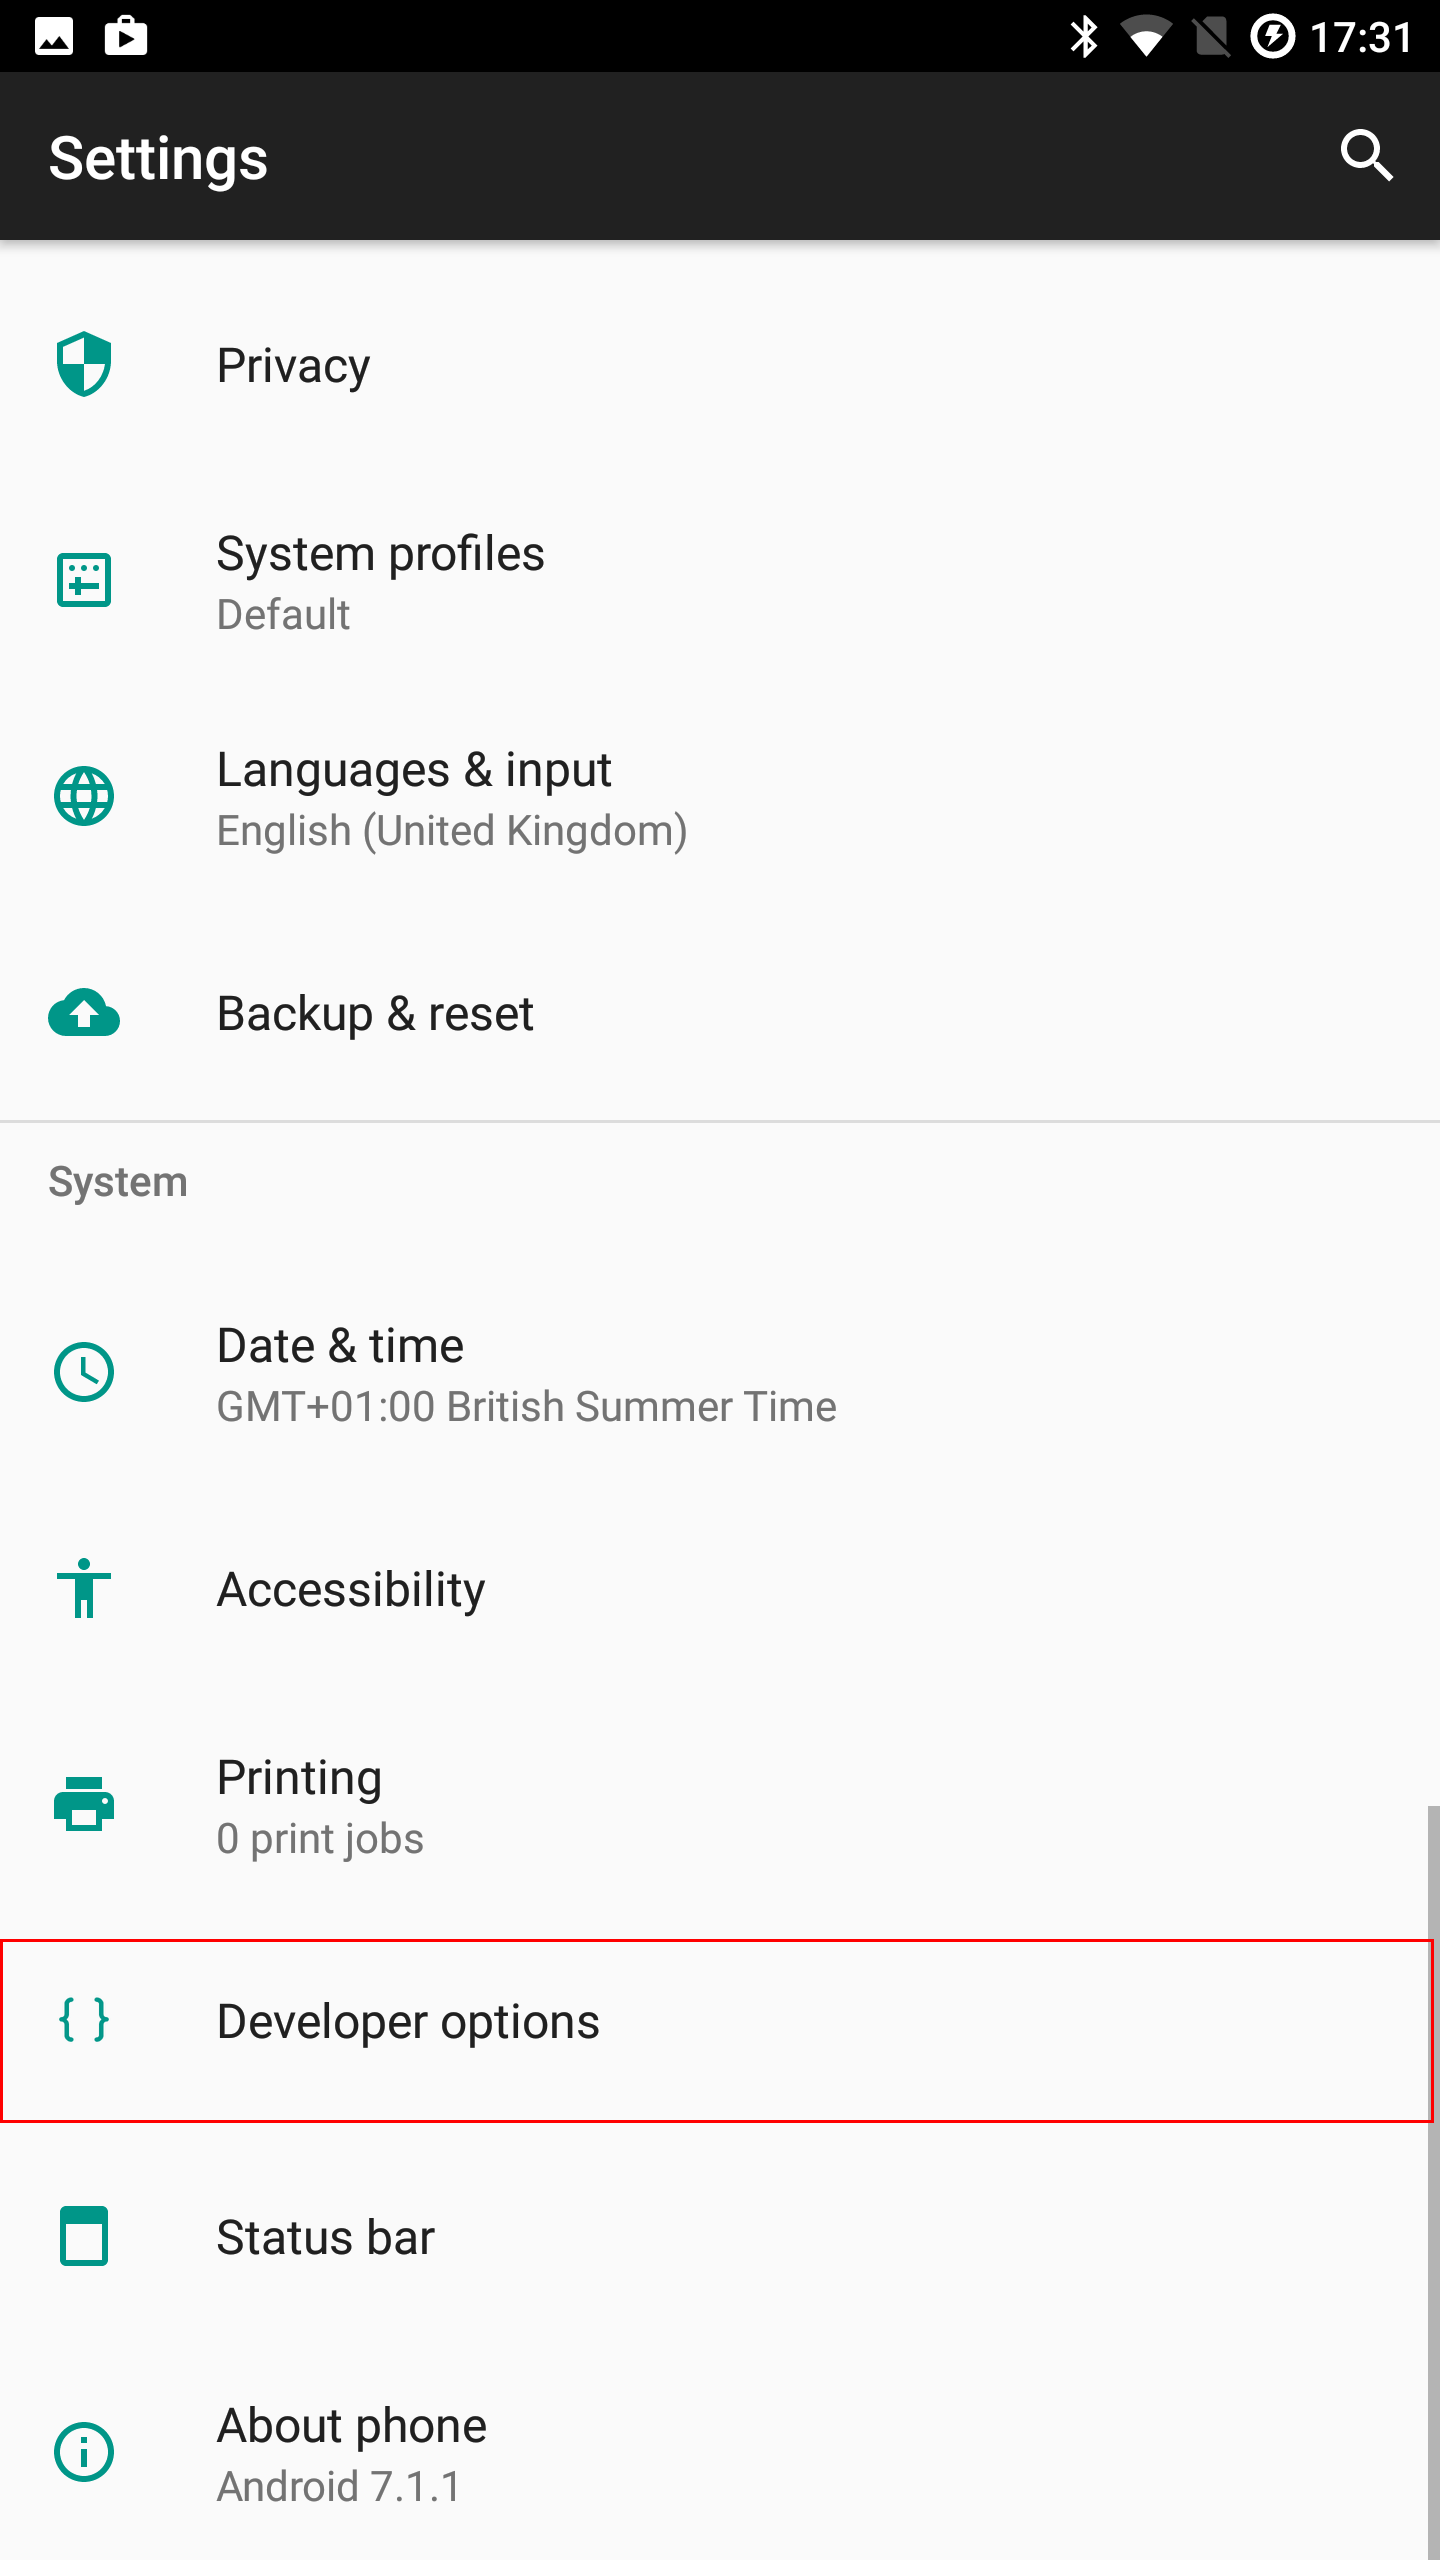
\includegraphics[scale=0.1]{Images/developerOption.png}}}
  \qquad
  \subfloat[Allow ADB message \label{fig:enableAdbMsg}]{{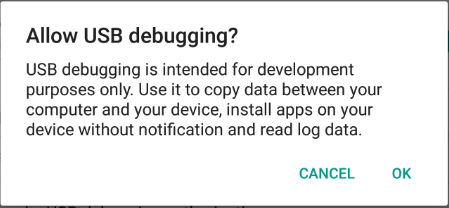
\includegraphics[scale=0.5]{./Images/allowAdbMsg.png}}}
  \caption{Enabling ADB on device}
  \label{fig:enablingADB}
\end{figure}

\begin{figure}
  \centering
  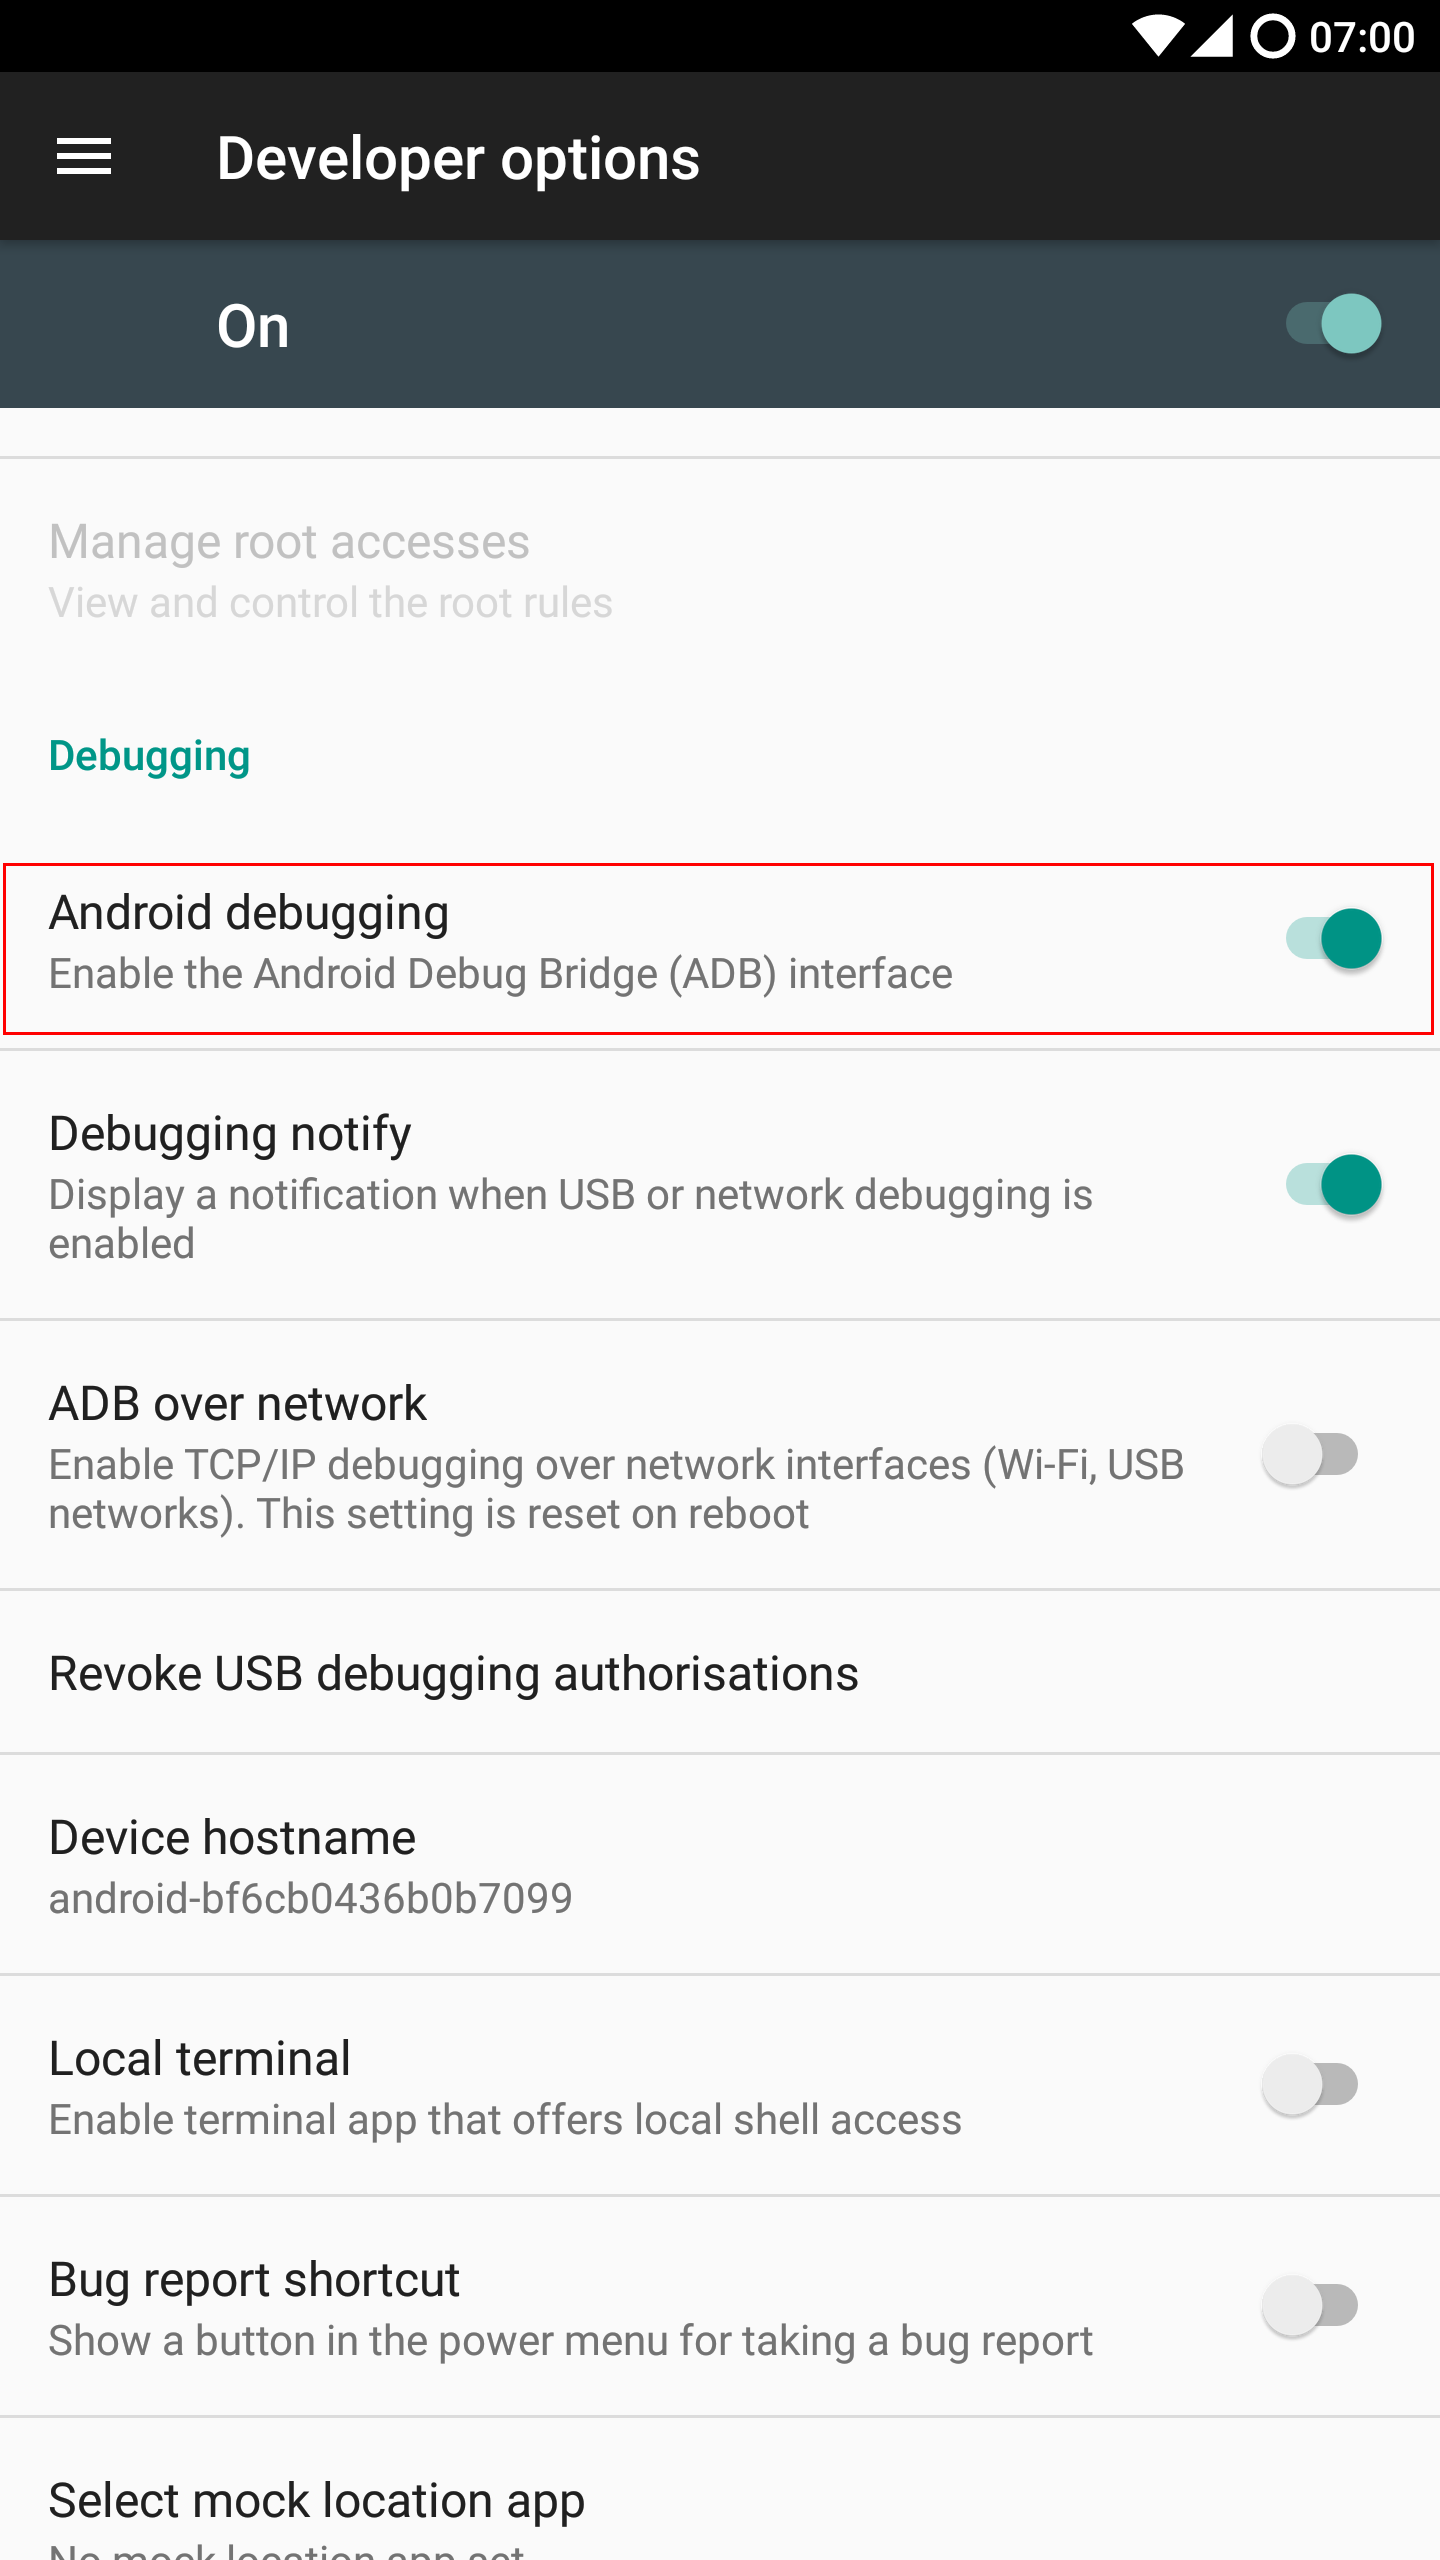
\includegraphics[scale=0.1]{Images/adbDebuggingOption.png}
  \caption{ADB option in developer menu}
  \label{fig:adbOption}
\end{figure}

\subsubsection{\texorpdfstring{Install ADB - \emph{Windows 10}
(Alternative
Installation)}{Install ADB - Windows 10 (Alternative Installation)}}\label{install-adb---windows-10-alternative-installation}

The installation of ADB will often be included with Android studio,
however to install ADB alone the easiest method would be to download and
use the ADB installer tool found on
\href{https://forum.xda-developers.com/showthread.php?t=2588979}{XDA-Developers}
\cite{AdbInstaller}.

Once installed running \lstinline!adb devices! will show all devices
connected to the computer with ADB enabled as shown in figure
\ref{fig:adbDevices}.

\begin{figure}
  \centering
  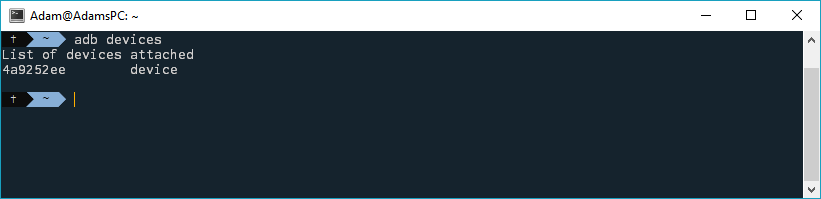
\includegraphics[scale=0.5]{Images/adbDevices.png}
  \caption{Results of running ADB devices command}
  \label{fig:adbDevices}
\end{figure}

\subsubsection{Installation via ADB (Alternative
Installation)}\label{installation-via-adb-alternative-installation}

Now that ADB is enabled on the device and installed on the computer it
is possible to run the command
\lstinline!adb install *apk file location*! passing in the location to
the apk file. If successful an installtion success message will be
displayed as shown in figure \ref{fig:adbSuccess}.

\begin{figure}[H]
  \centering
  \subfloat[ADB install command]{{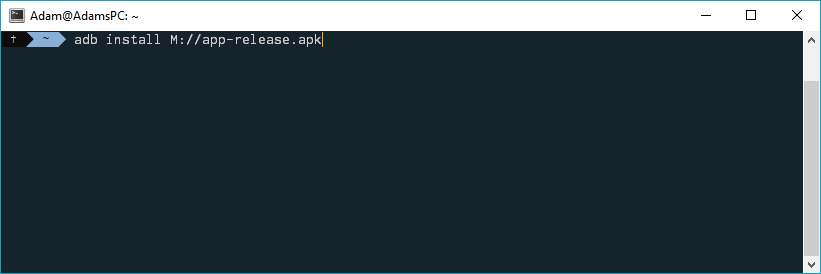
\includegraphics[scale=0.5]{./Images/adbInstall.png}}}
  \qquad
  \subfloat[Results of application installation success]{{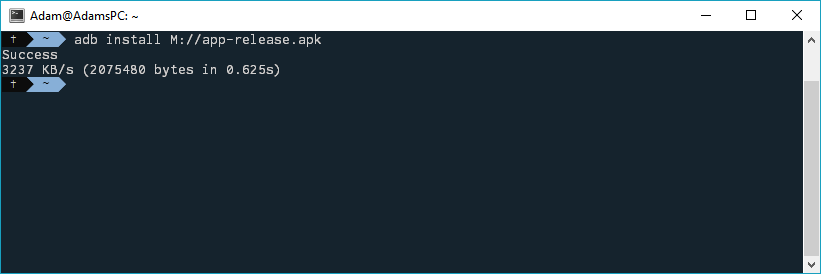
\includegraphics[scale=0.5]{./Images/adbInstallSuccess.png}}}
  \caption{Installing APK using ADB}
  \label{fig:adbSuccess}
\end{figure}

\subsection{Alarms}\label{alarms}

This section will provide instructions for the functionality of the
alarm functionality.

\subsubsection{Create}\label{create}

By clicking on the alarm create button at the bottom of the screen (as
seen in figure \ref{fig:addAlarm}) a time picker dialog will appear.

\begin{figure}[H]
  \centering
  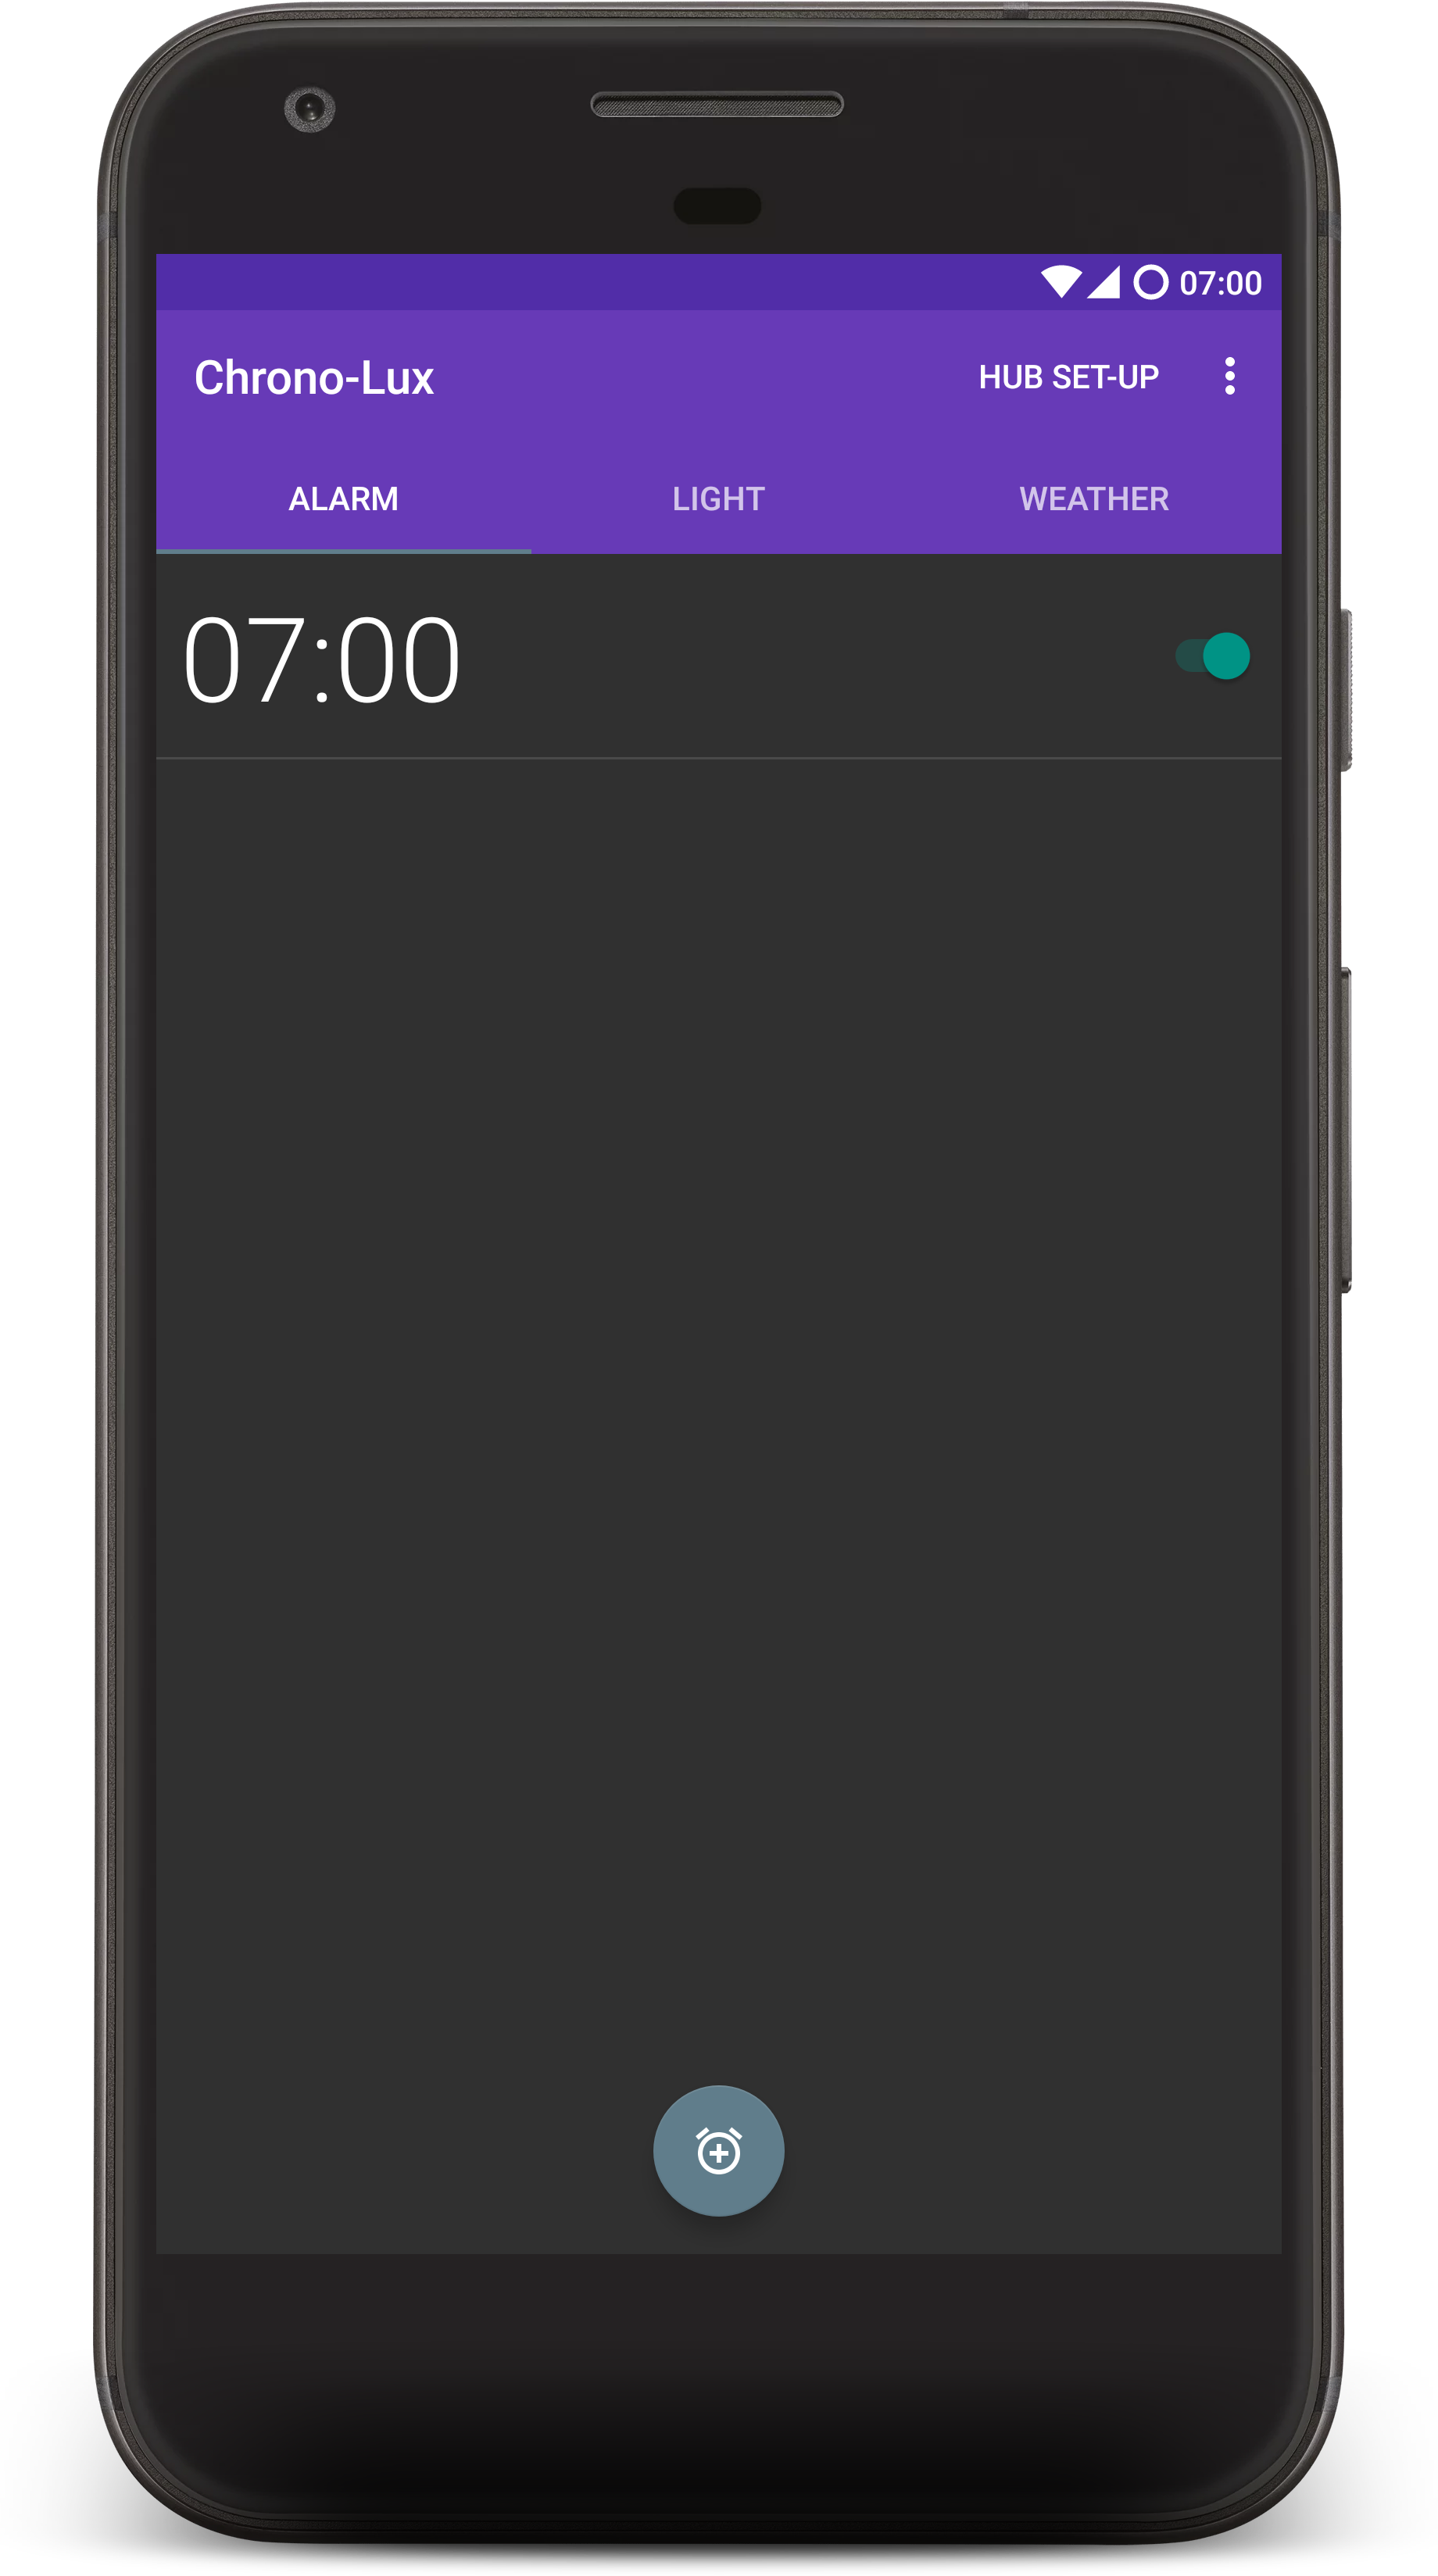
\includegraphics[scale=0.1]{Images/addAlarm.png}
  \caption{Create alarm button}
  \label{fig:addAlarm}
\end{figure}

First the hour will be selected, to select the hour desired for the
alarm either tap on time or for more precision, press and drag the
\emph{hand} of the clock to the desired time. When released the picker
will now allow for the selection of the minutes; repeat the same action
as for the hour to select the chosen time.

\subsubsection{Rename}\label{rename}

Renaming an alarm is simple, by taping the alarm that needs renaming an
edit text pop-up will appear (as seen in figure \ref{fig:changeLabel});
enter the new label desired and confirm the change, the alarm is now
called something else.

\begin{figure}[H]
  \centering
  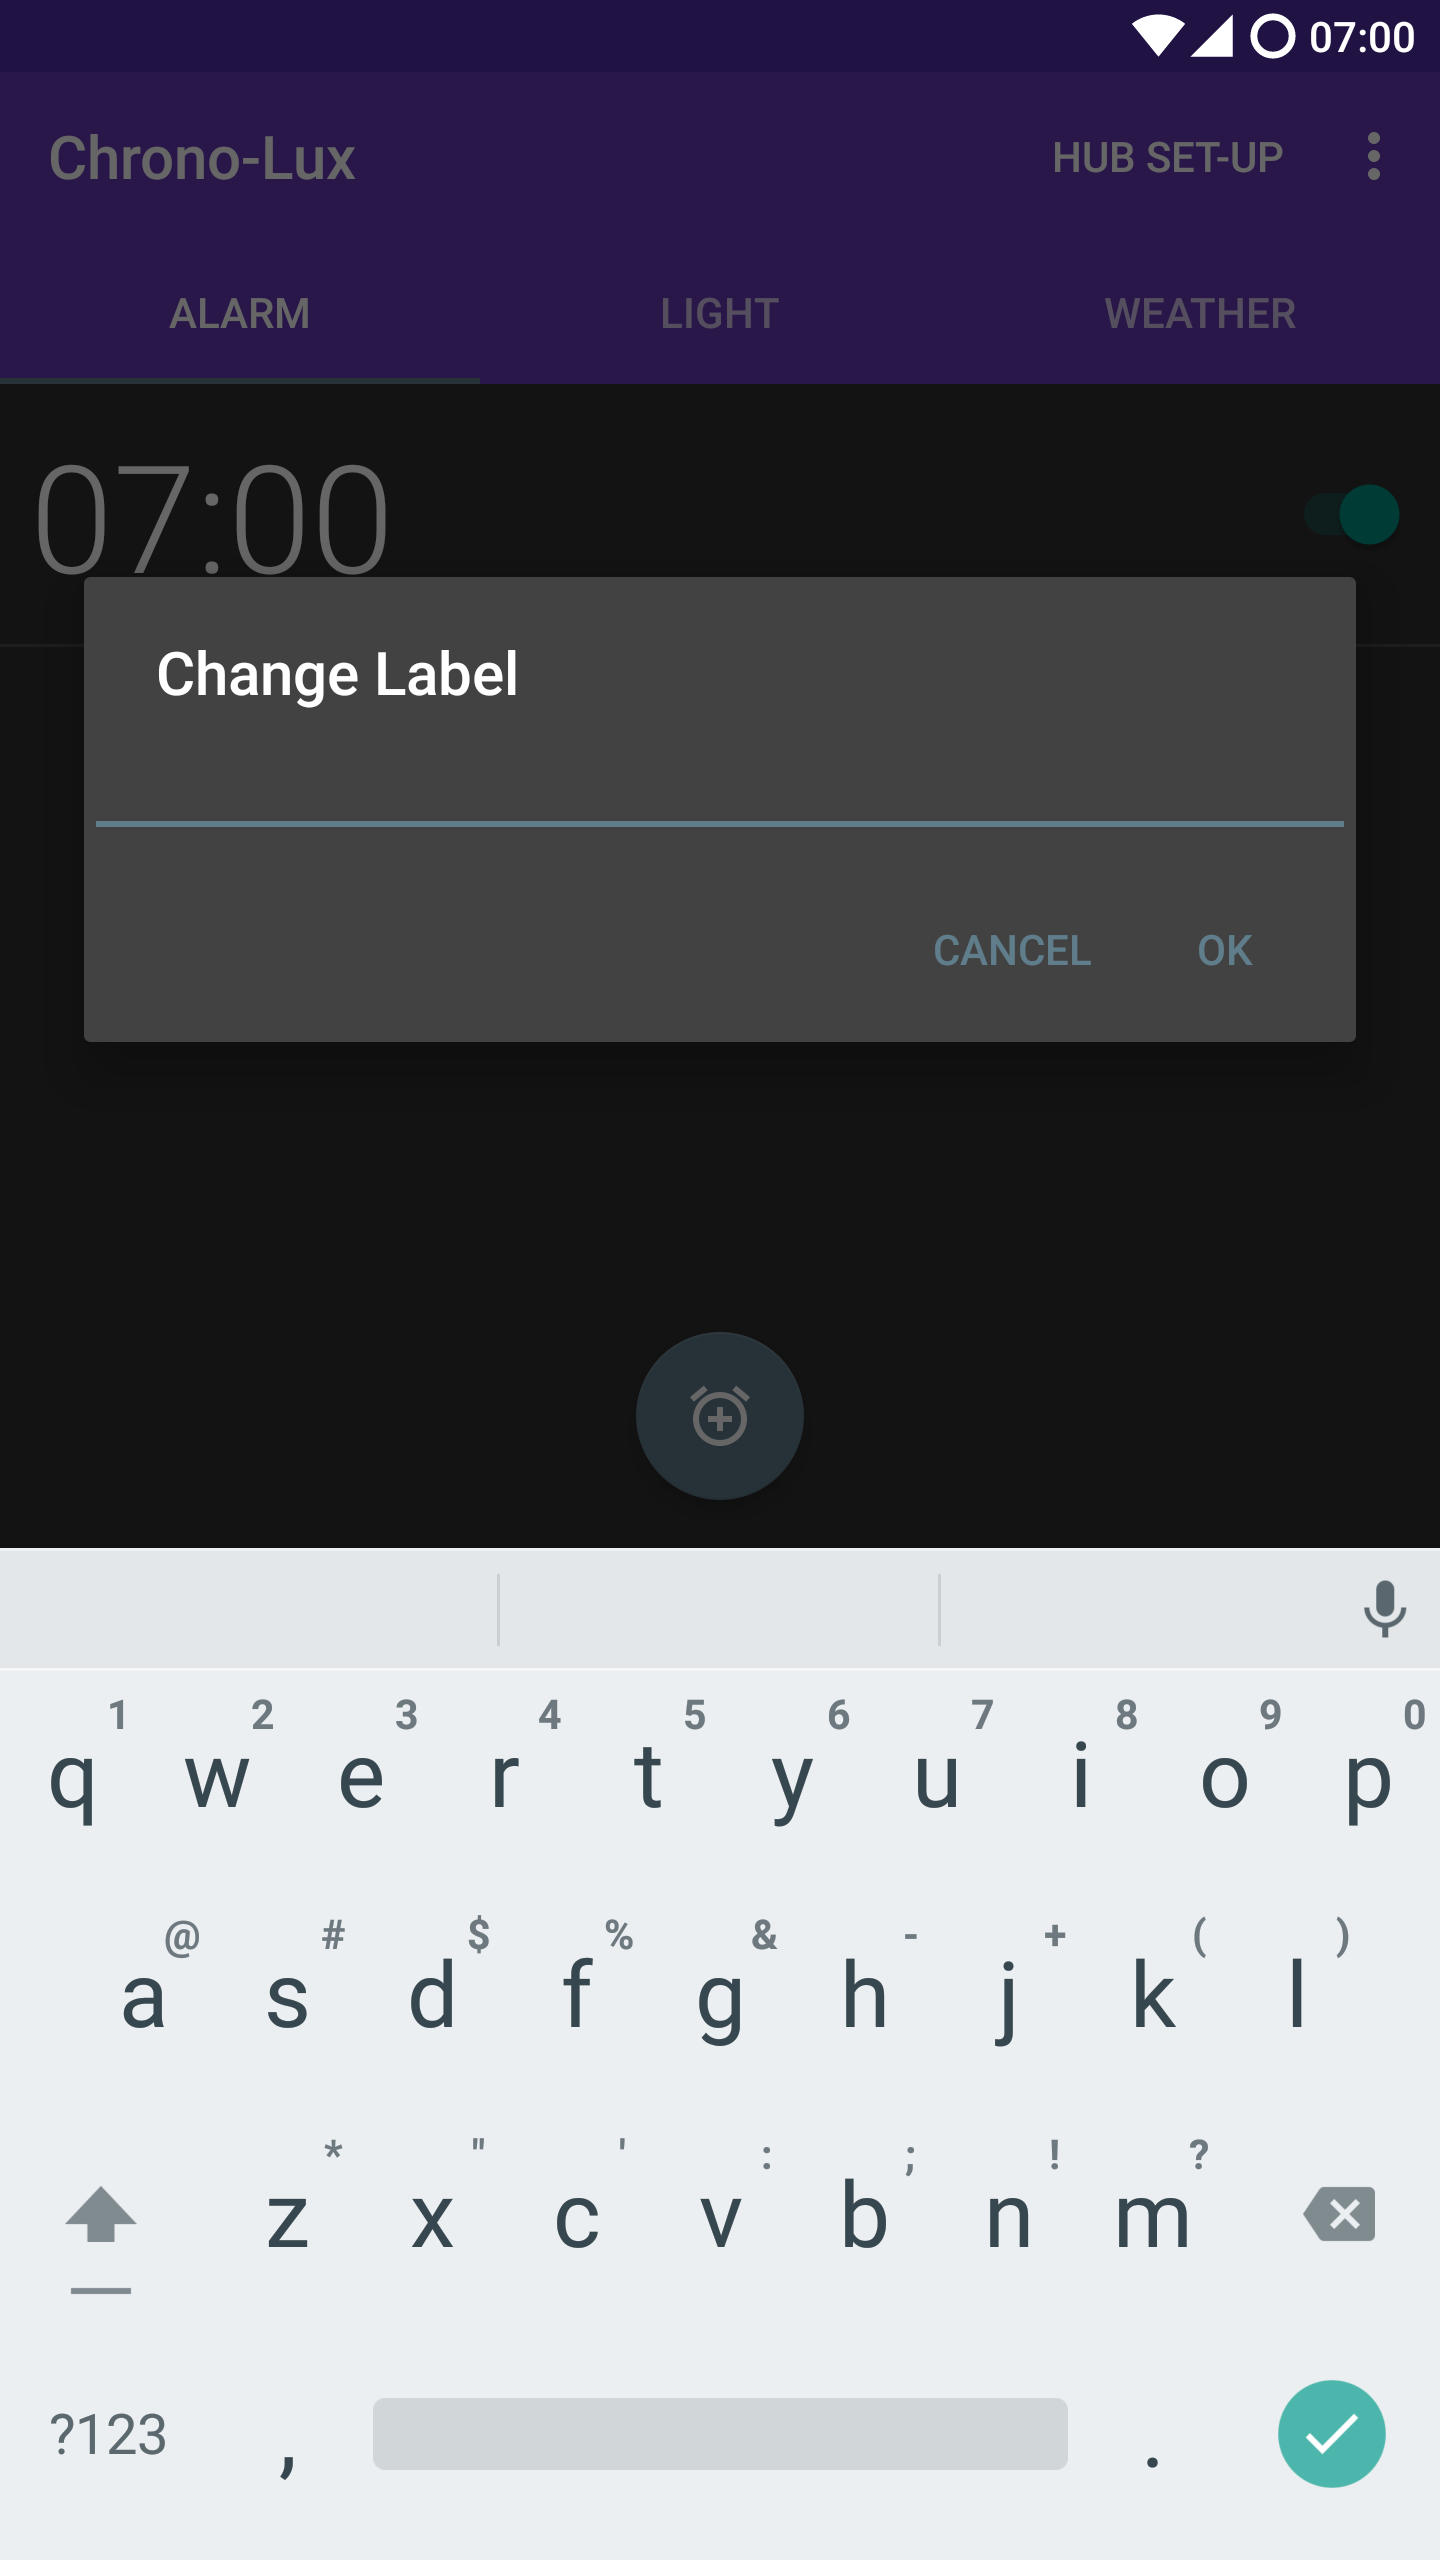
\includegraphics[scale=0.1]{Images/changeLabel.png}
  \caption{Change label edit text}
  \label{fig:changeLabel}
\end{figure}

The label provided to the alarm will appear when the alarm goes off and
be displayed in the alarm notification.

\subsubsection{Turning Off/On an Alarm}\label{turning-offon-an-alarm}

By pressing the switch on the right hand side of the screen, it is
possible to toggle the alarm on or off.

\begin{figure}[H]
  \centering
  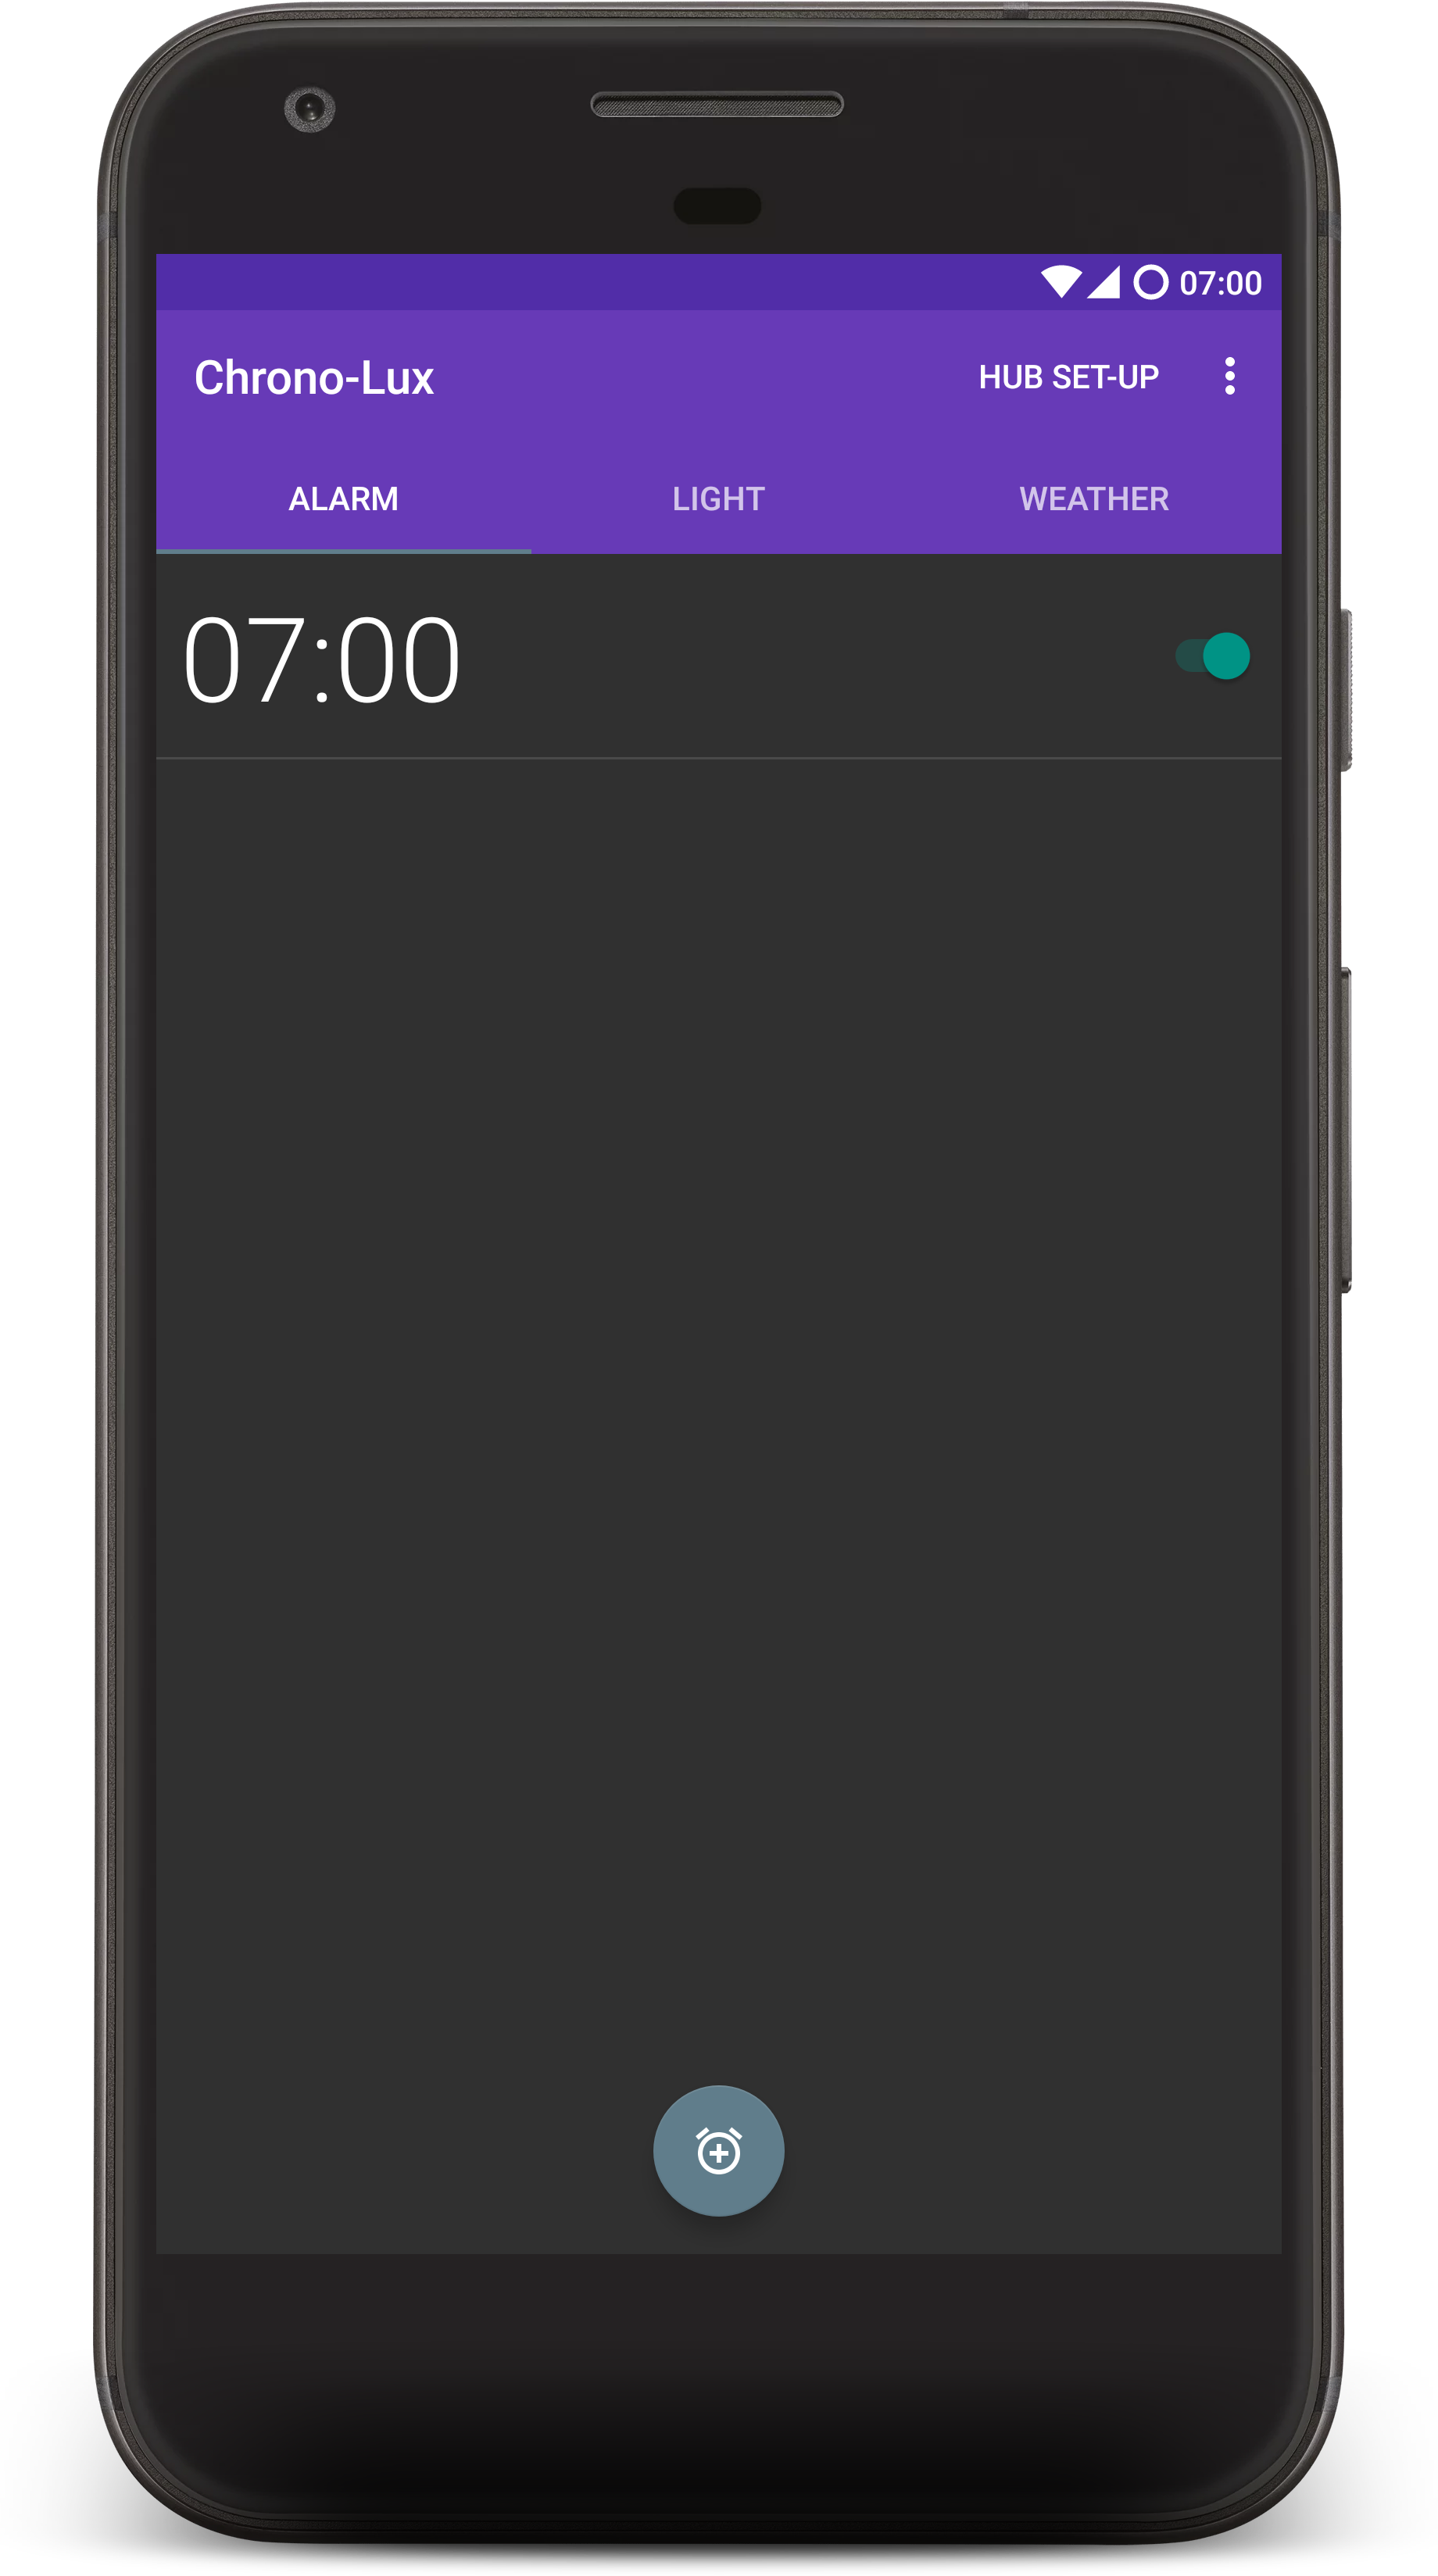
\includegraphics[trim= 0 2000 0 0, clip, scale=0.1]{Images/addAlarm.png}
  \caption{Toggle alarm switch}
  \label{fig:toggleAlarm}
\end{figure}

\subsubsection{Delete}\label{delete}

To delete and existing alarm, simply press and hold the alarm to be
deleted, a prompt will appear asking to confirm the action.

\begin{figure}[H]
  \centering
  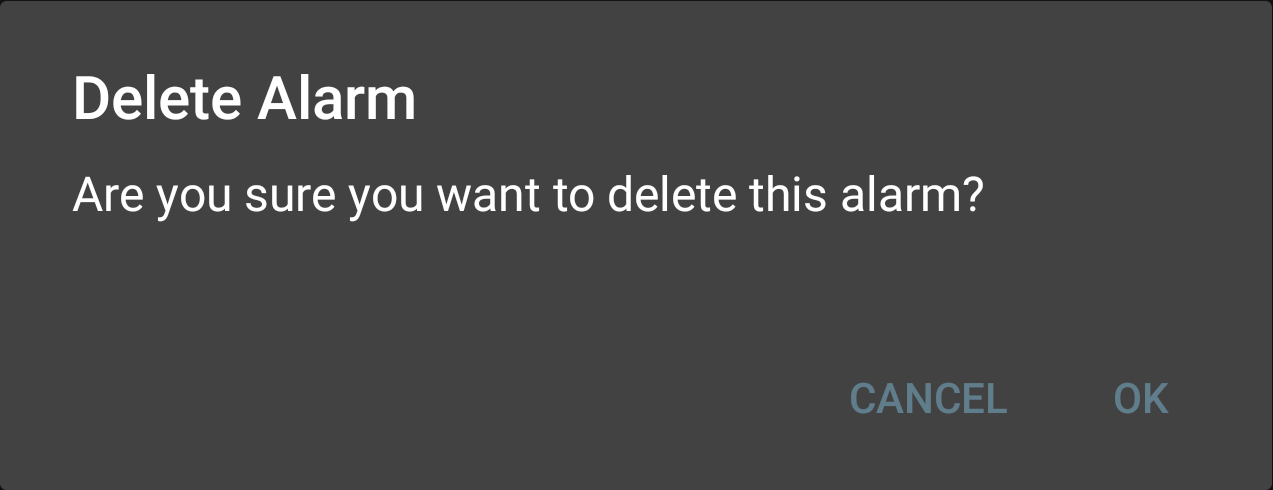
\includegraphics[scale=0.2]{Images/deleteAlarmDialog.png}
  \caption{Delete alarm dialog box}
  \label{fig:deleteAlarm}
\end{figure}

\subsection{Lights}\label{lights}

It is required to connect the application to a lighting bridge to be
able to enable the lighting functionality within the application. The
alarms and weather will work without the lighting being configured.

\subsubsection{Connecting to the Bridge}\label{connecting-to-the-bridge}

To be able to use the smart-light functionality it is necessary to pair
the application with the bridge prior to use, this allows the
application to be \emph{white-listed} and provide access to the lighting
interface.

When navigating to the lighting tab, if no bridge has been configured a
text prompt will appear and at the press of the button will take you to
the set-up activity. If the activity does not automatically begin
searching for a bridge, pressing the search for bridge button will begin
a search.

\begin{figure}[H]
  \centering
  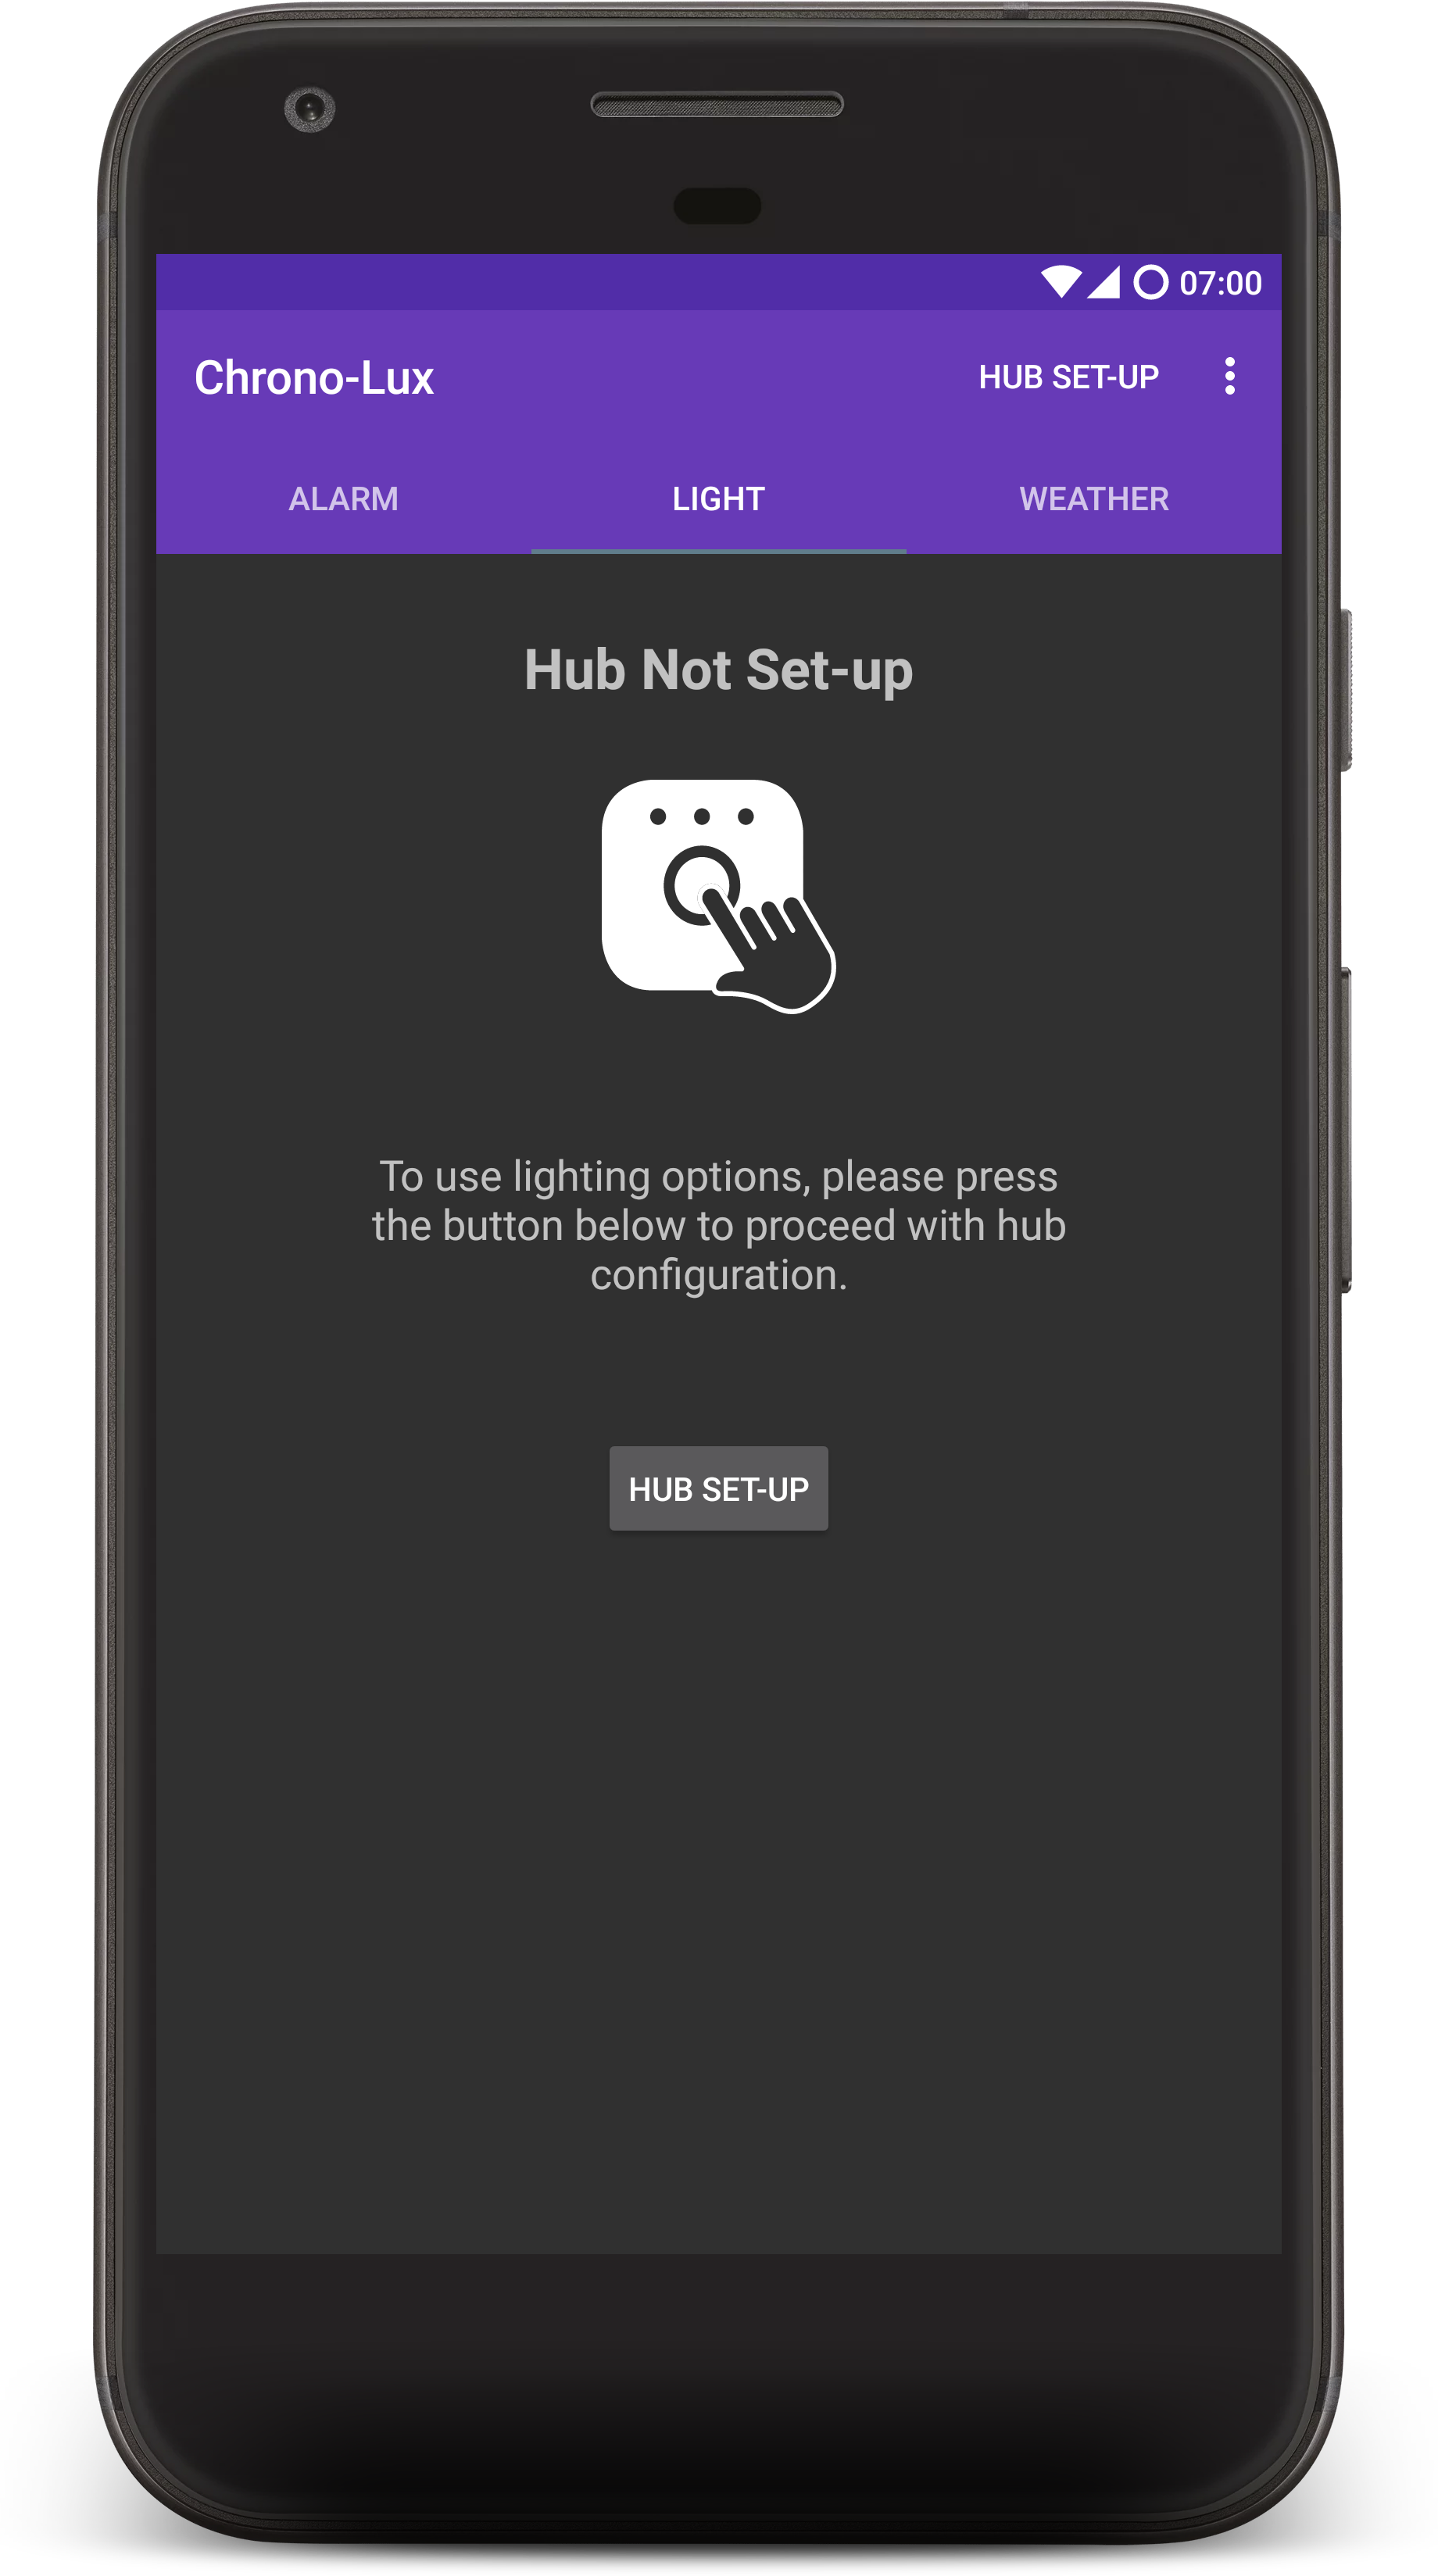
\includegraphics[scale=0.1]{Images/setupPrompt.png}
  \caption{Bridge set-up prompt screen}
  \label{fig:setupPrompt}
\end{figure}

If no bridges are returned please ensure you are on the same local
network as the bridge and there are no firewalls, VPNs or other
potential network configuration that could be blocking communications.
If no bridges are found or you would like to search again, simply press
the search button again.

\begin{figure}[H]
  \centering
  \subfloat[Searching for bridge]{{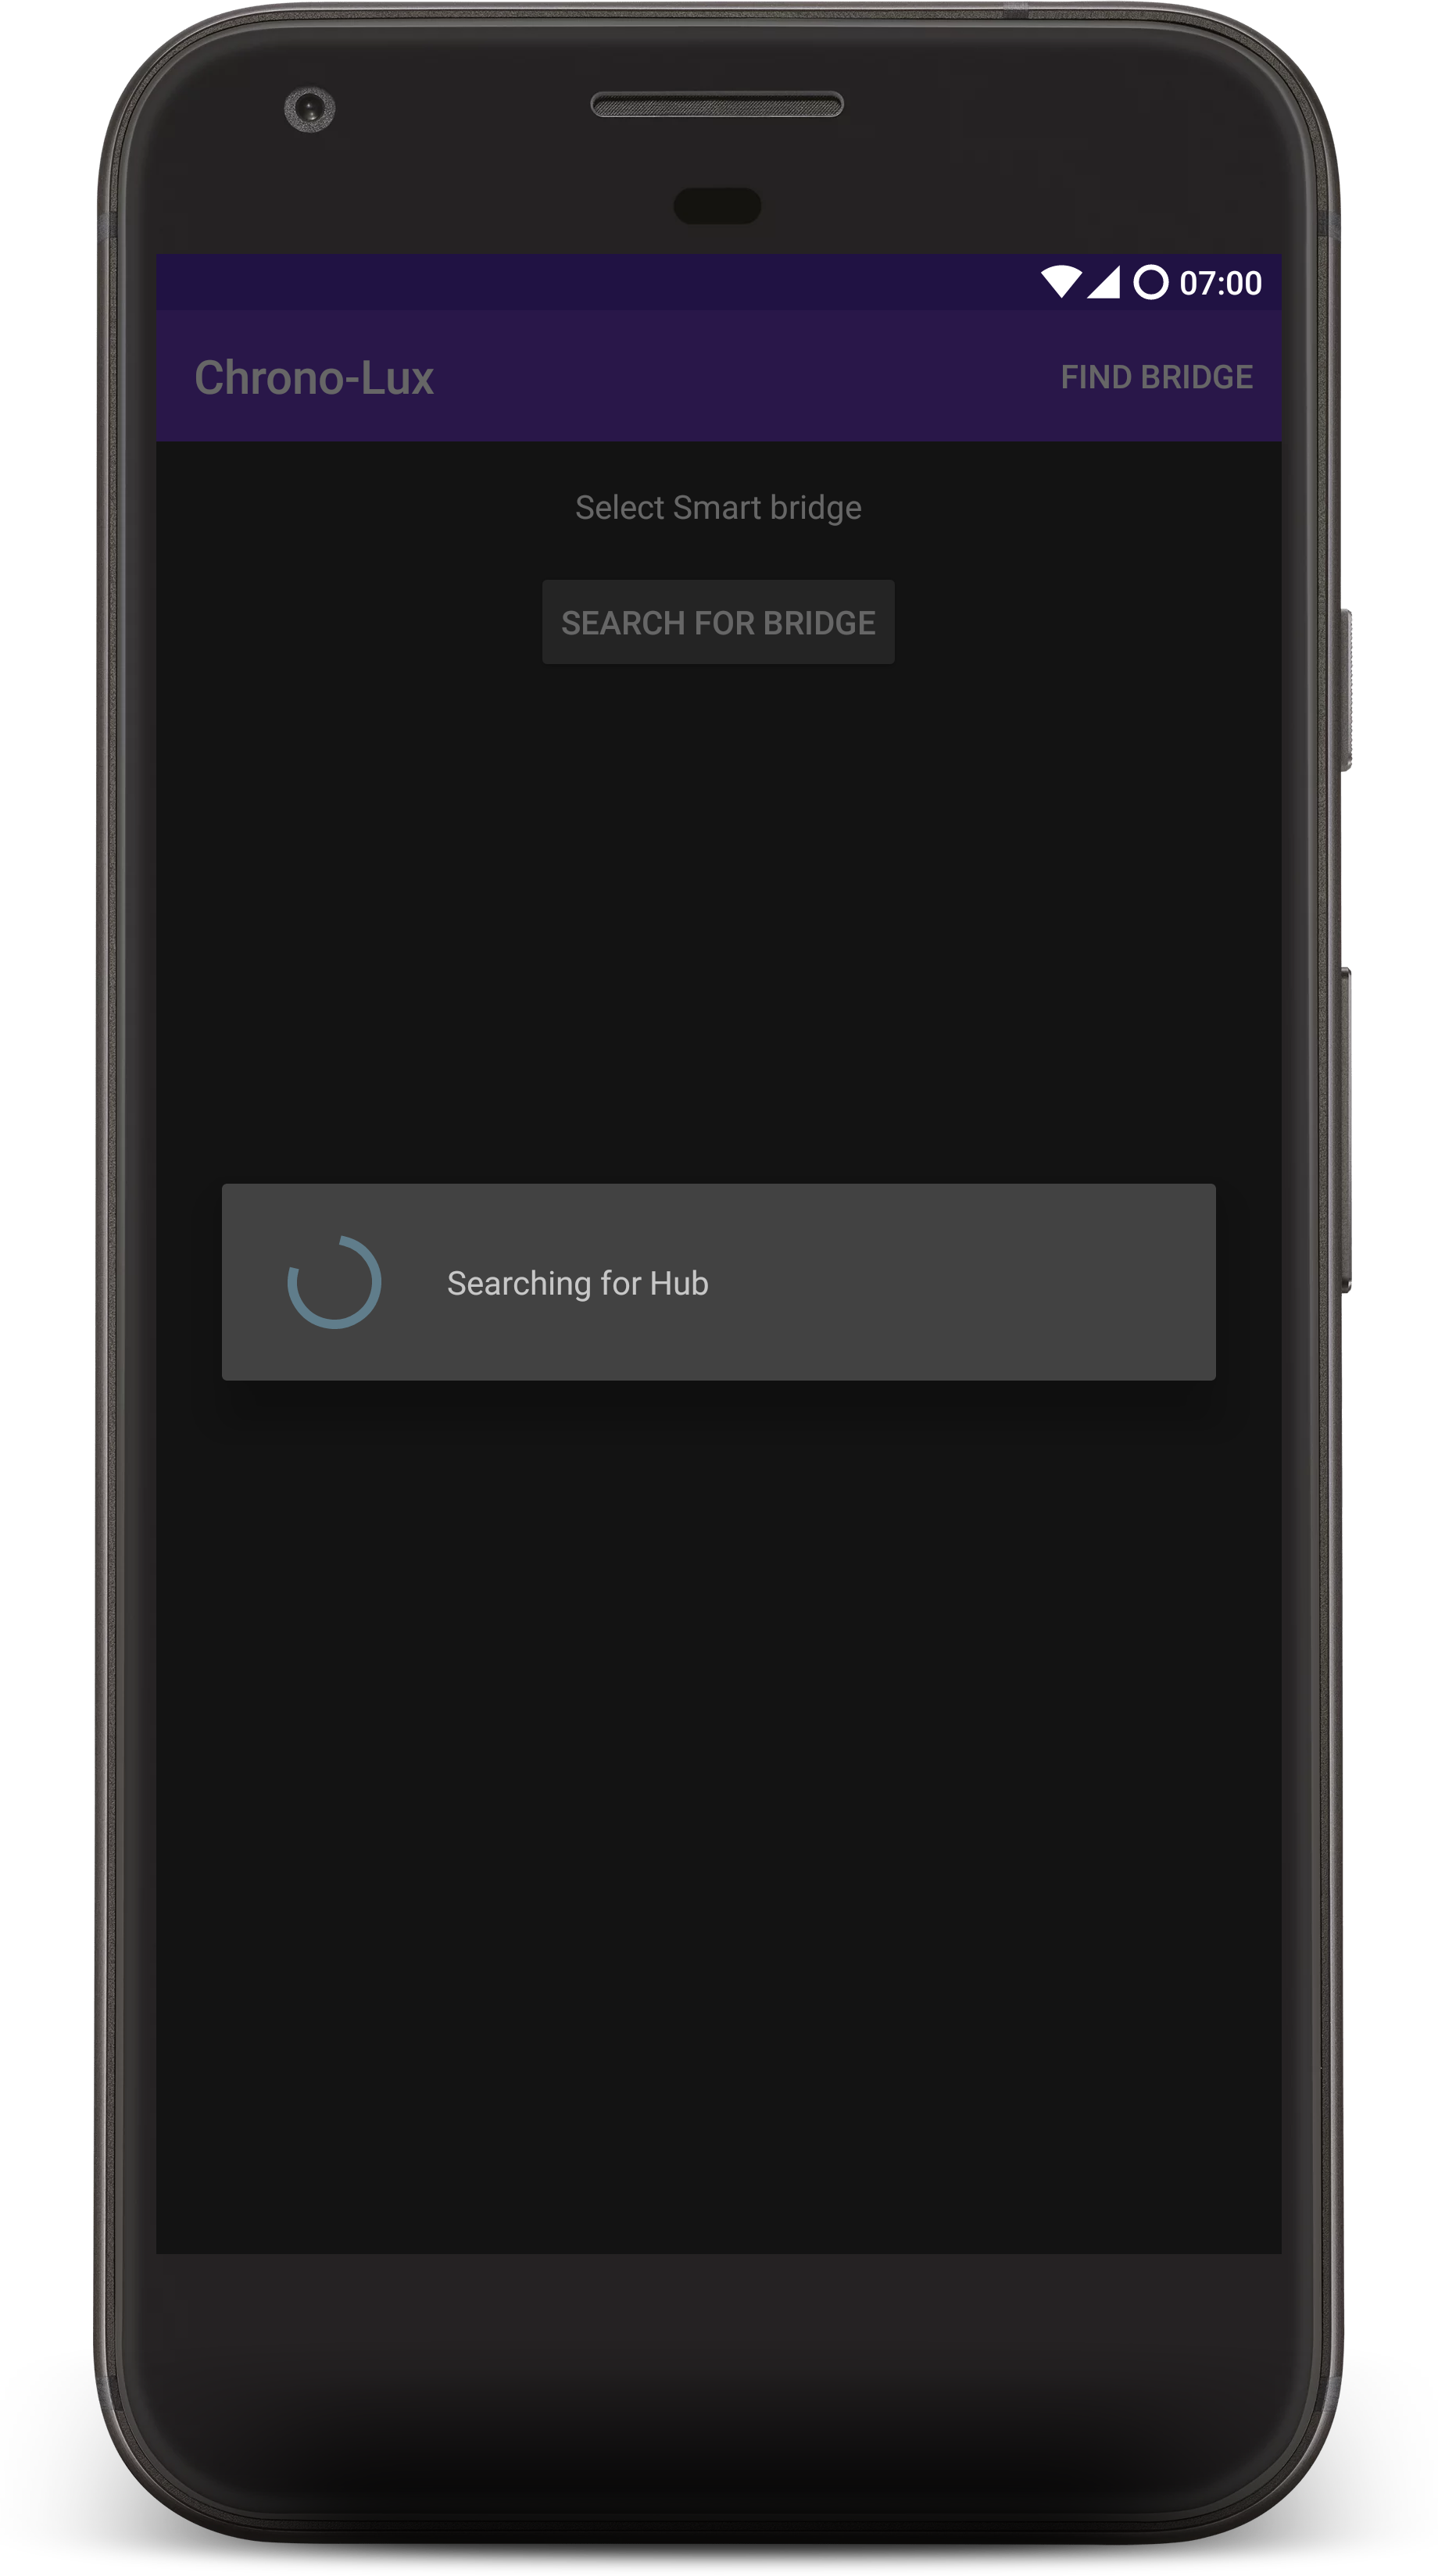
\includegraphics[scale=0.09]{./Images/searchingForHub.png}}}
  \qquad
  \subfloat[Bridge connection error]{{
\includegraphics[scale=0.2]{Images/bridgeError.png}}}
  \caption{Finding available bridges}%
  \label{fig:searchForBridge}%
\end{figure}

When the search is completed a list of all found bridges will be
displayed, to select one tap on it to begin the authentication process.

\begin{figure}[H]
  \centering
  \subfloat[No bridge found screen]{{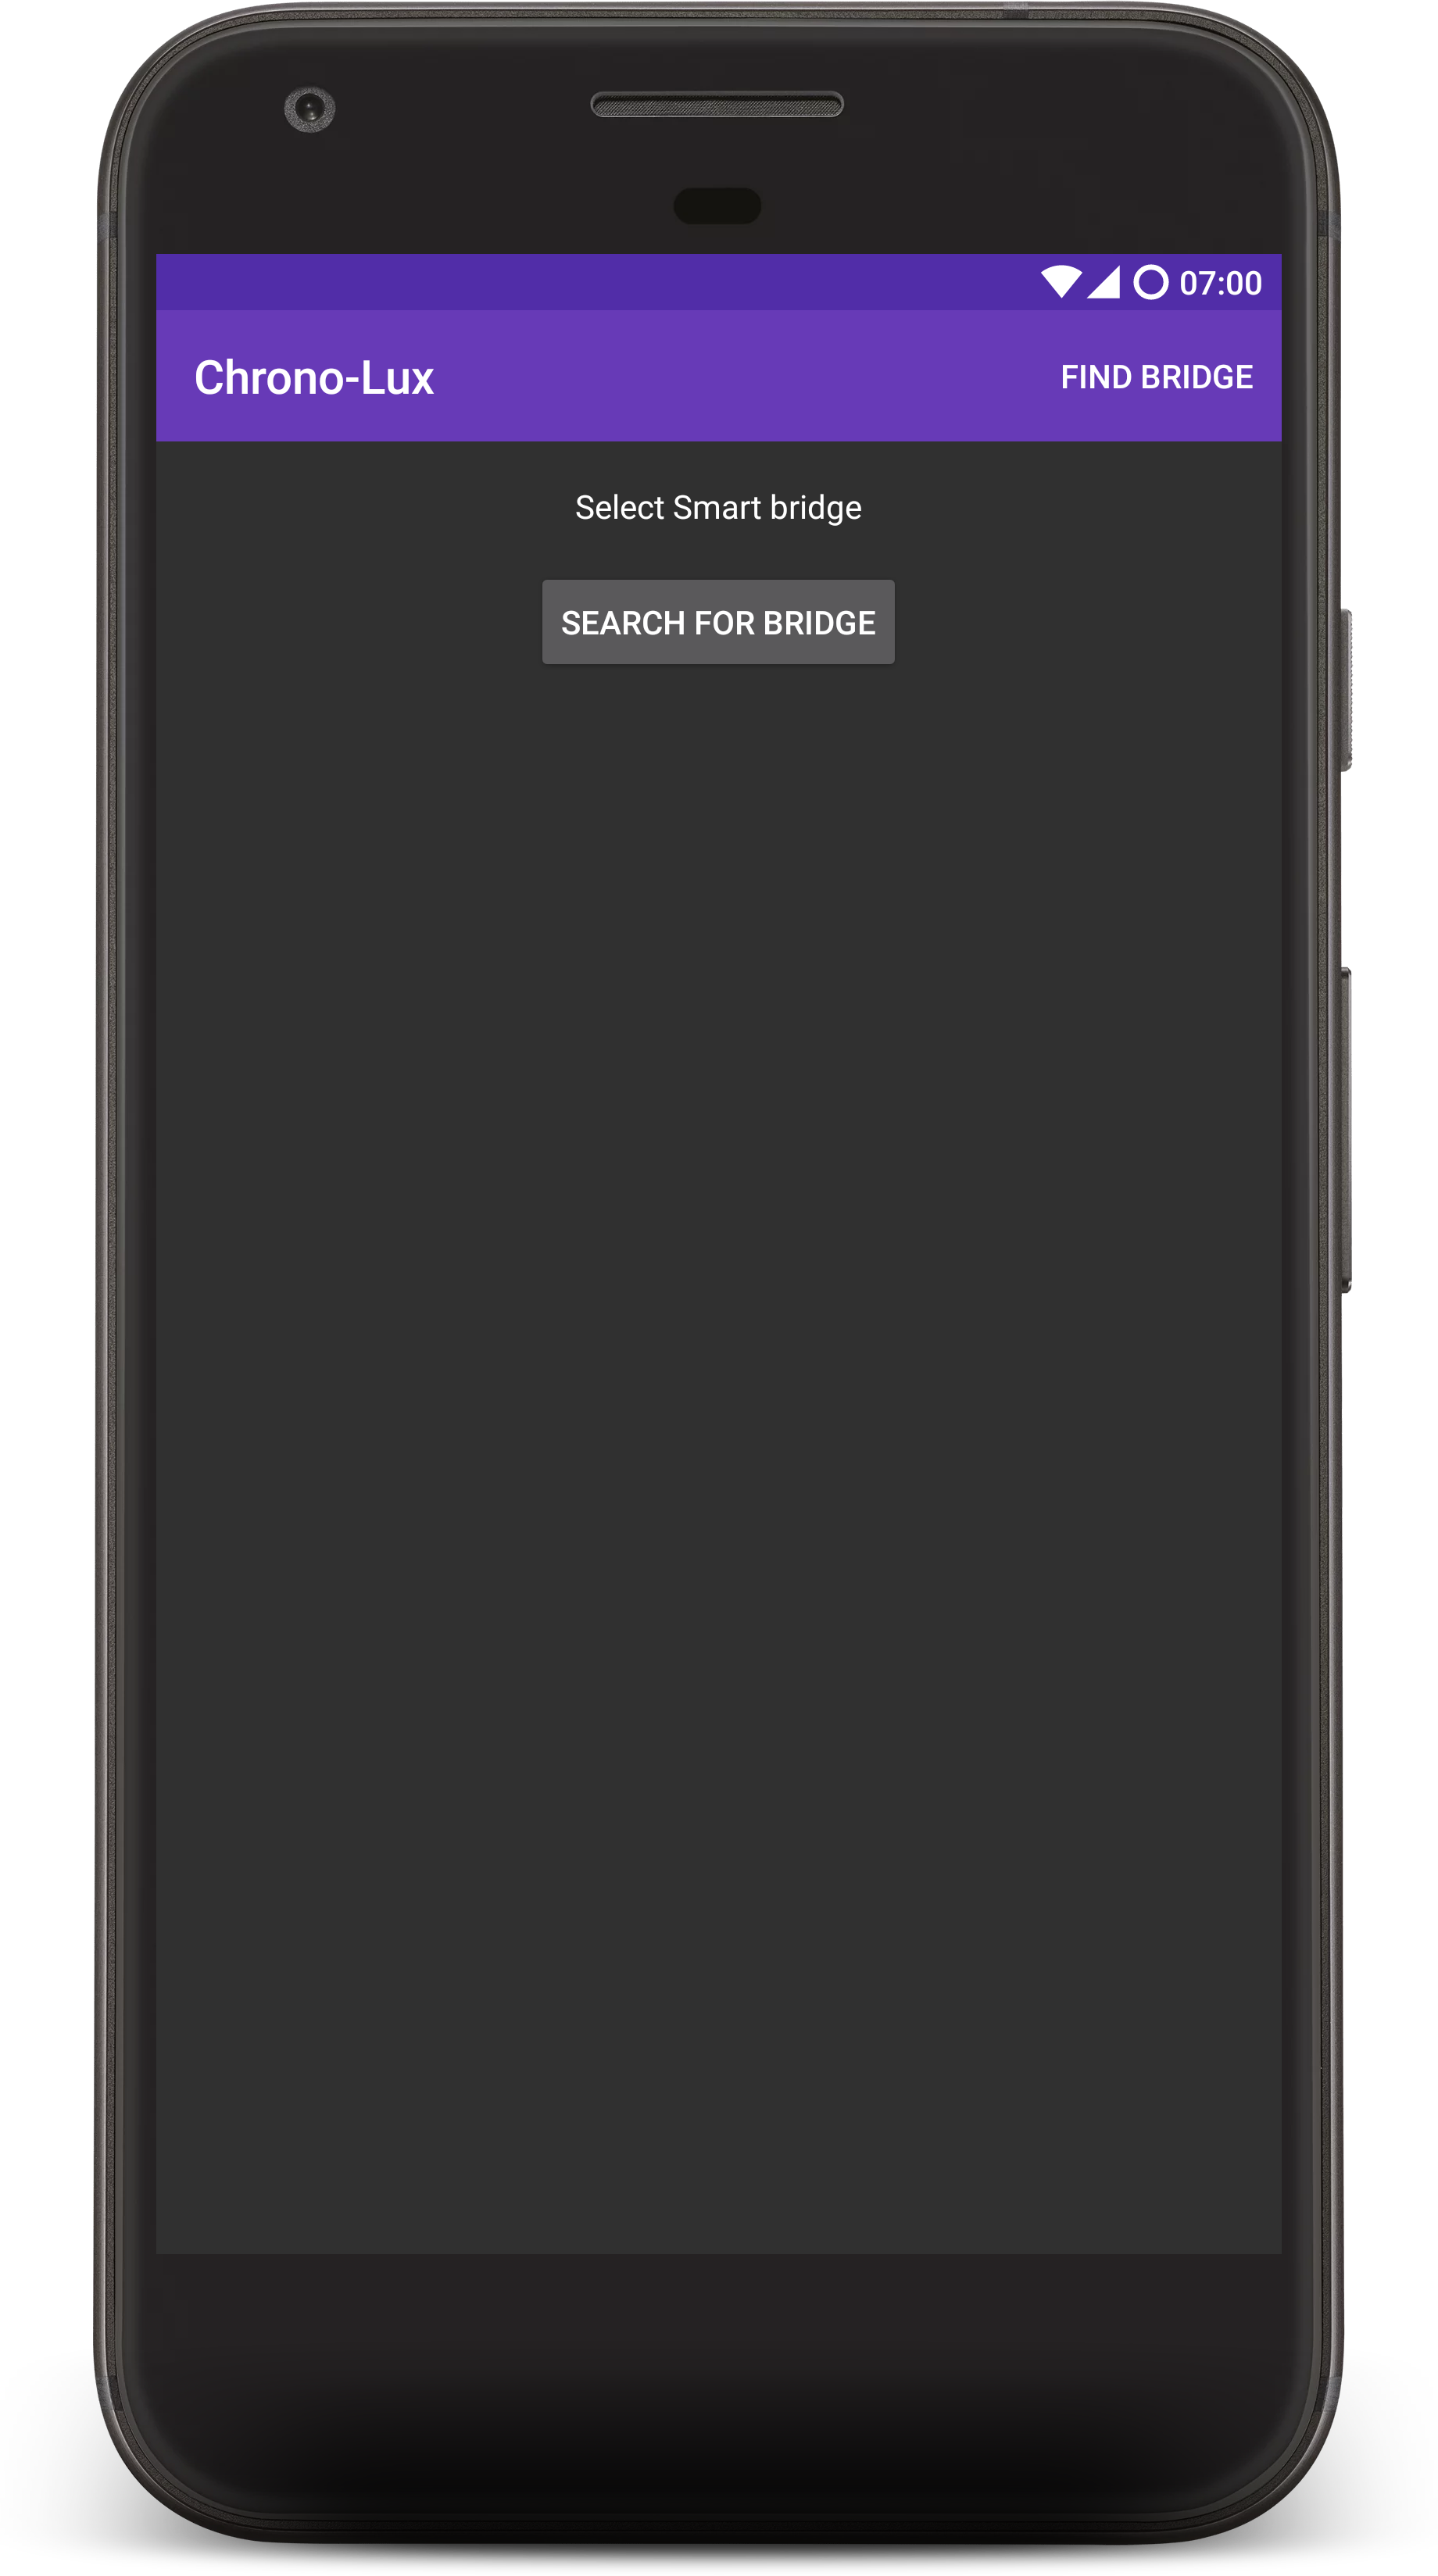
\includegraphics[trim= 0 2000 0 0, clip, scale=0.09]{./Images/noBridgeFound.png}}}
  \qquad
  \subfloat[List of available bridges]{{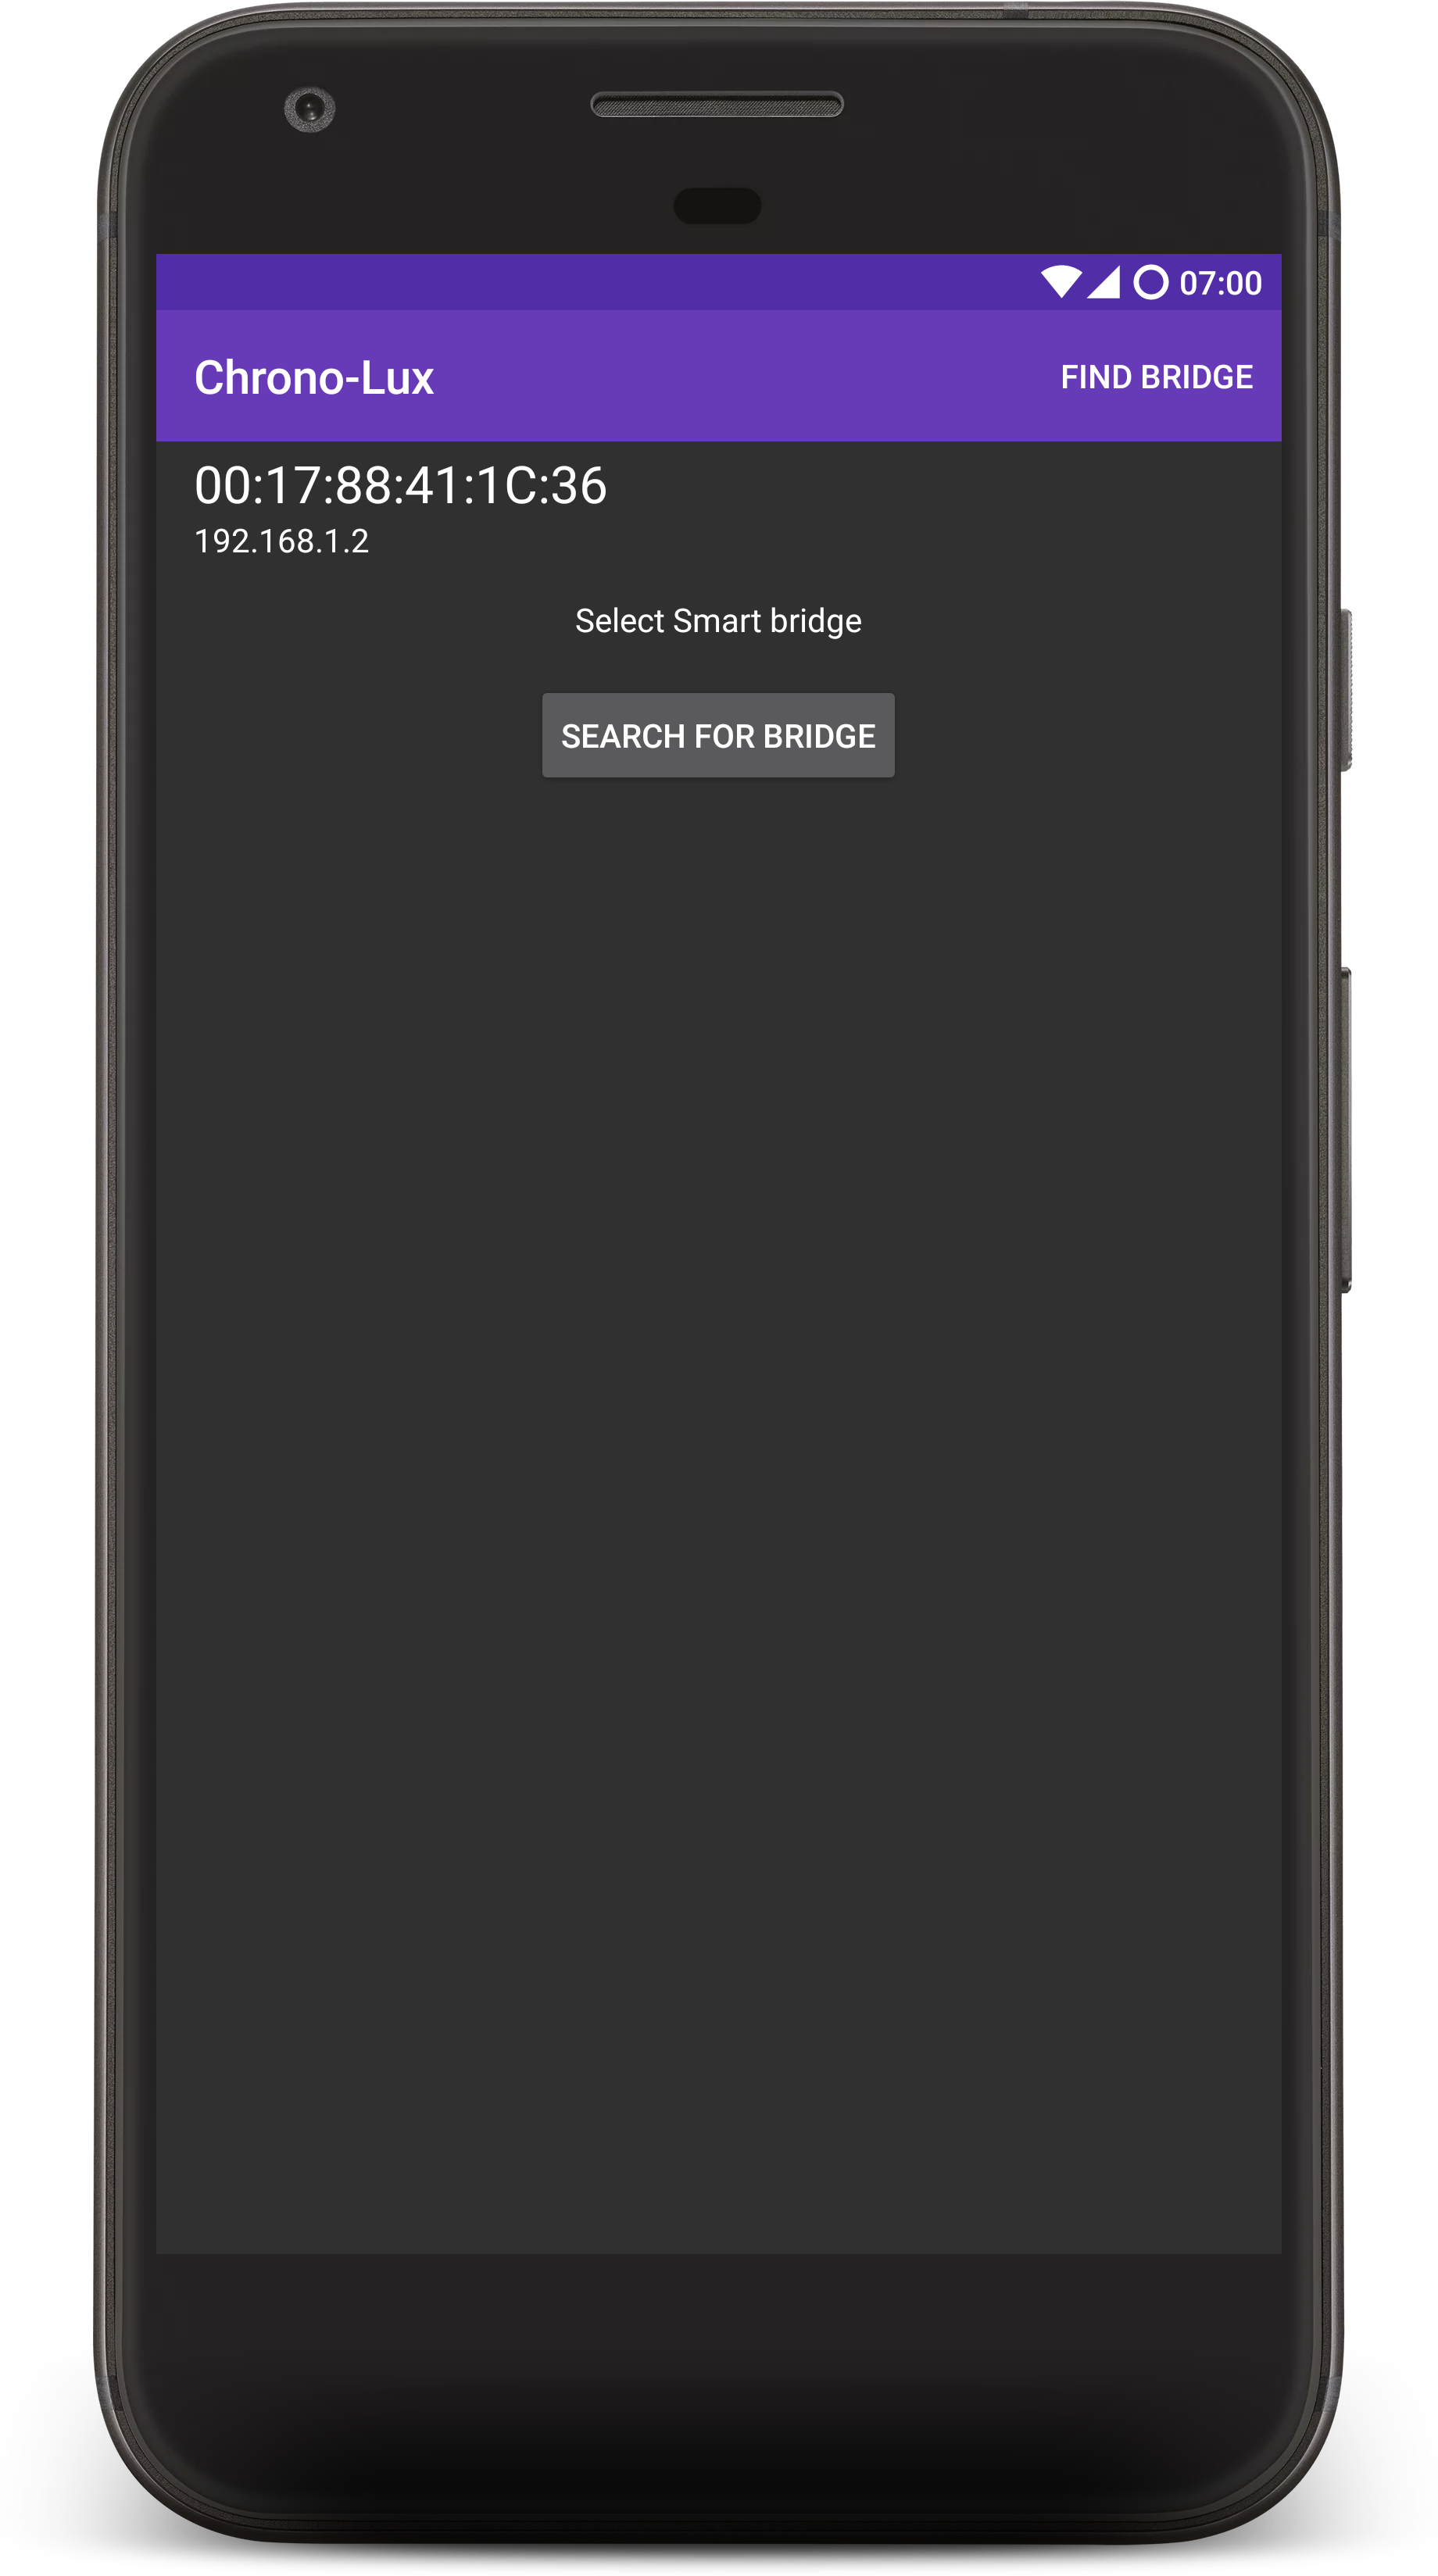
\includegraphics[trim= 0 2000 0 0, clip, scale=0.09]{./Images/bridgeList.png}}}
  \caption{Finding available bridges}
  \label{fig:findBridge}%
\end{figure}

On selecting a bridge the push-button authentication will occur, please
press the large push-link button on the front/top of the bridge. This
action is to ensure that there is physical access to the bridge as a
security measure to prevent un-authorised applications or intruders on
the network gaining access to the lighting interface.

\begin{figure}[H]
  \centering
  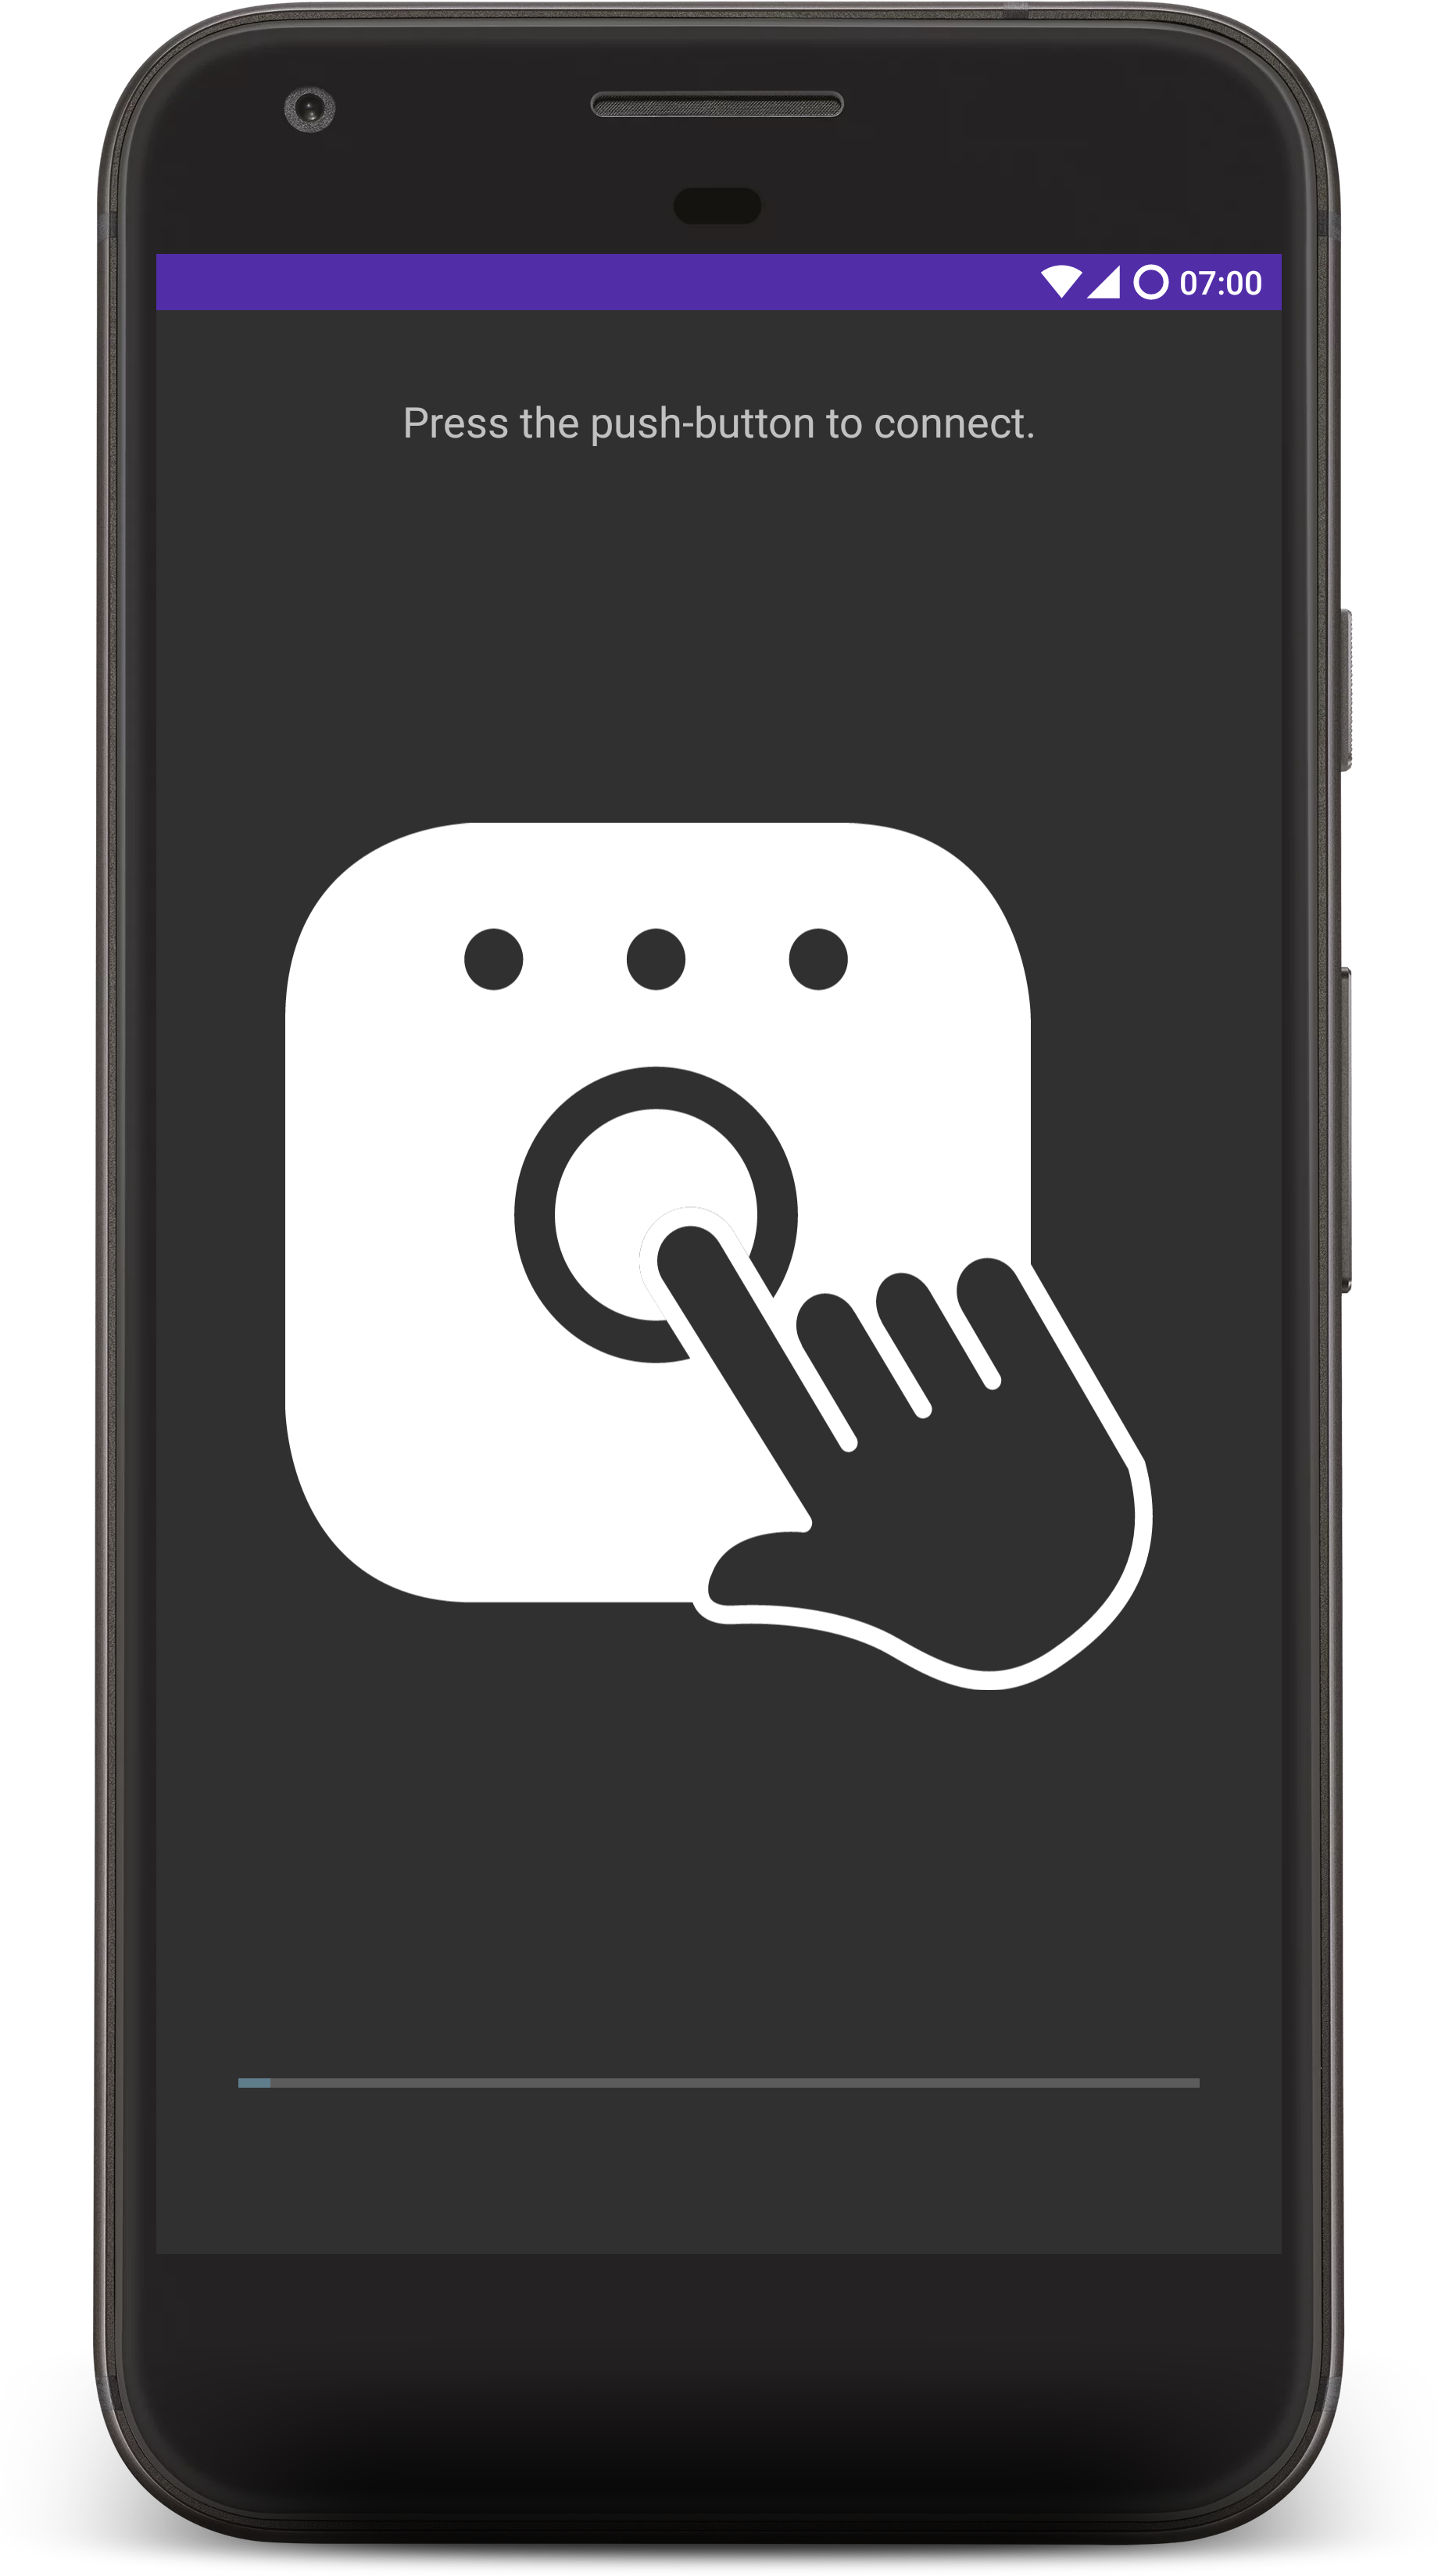
\includegraphics[scale=0.09]{Images/pushLinkScreen.png}
  \caption{The push-link prompt and countdown}
  \label{fig:pushPrompt}
\end{figure}

On successful authentication you shall be returned back to the main
application, now when navigating to the lighting tab any connected
lights shall be displayed similar to that shown in figure
\ref{fig:lightList}.

\begin{figure}[H]
  \centering
  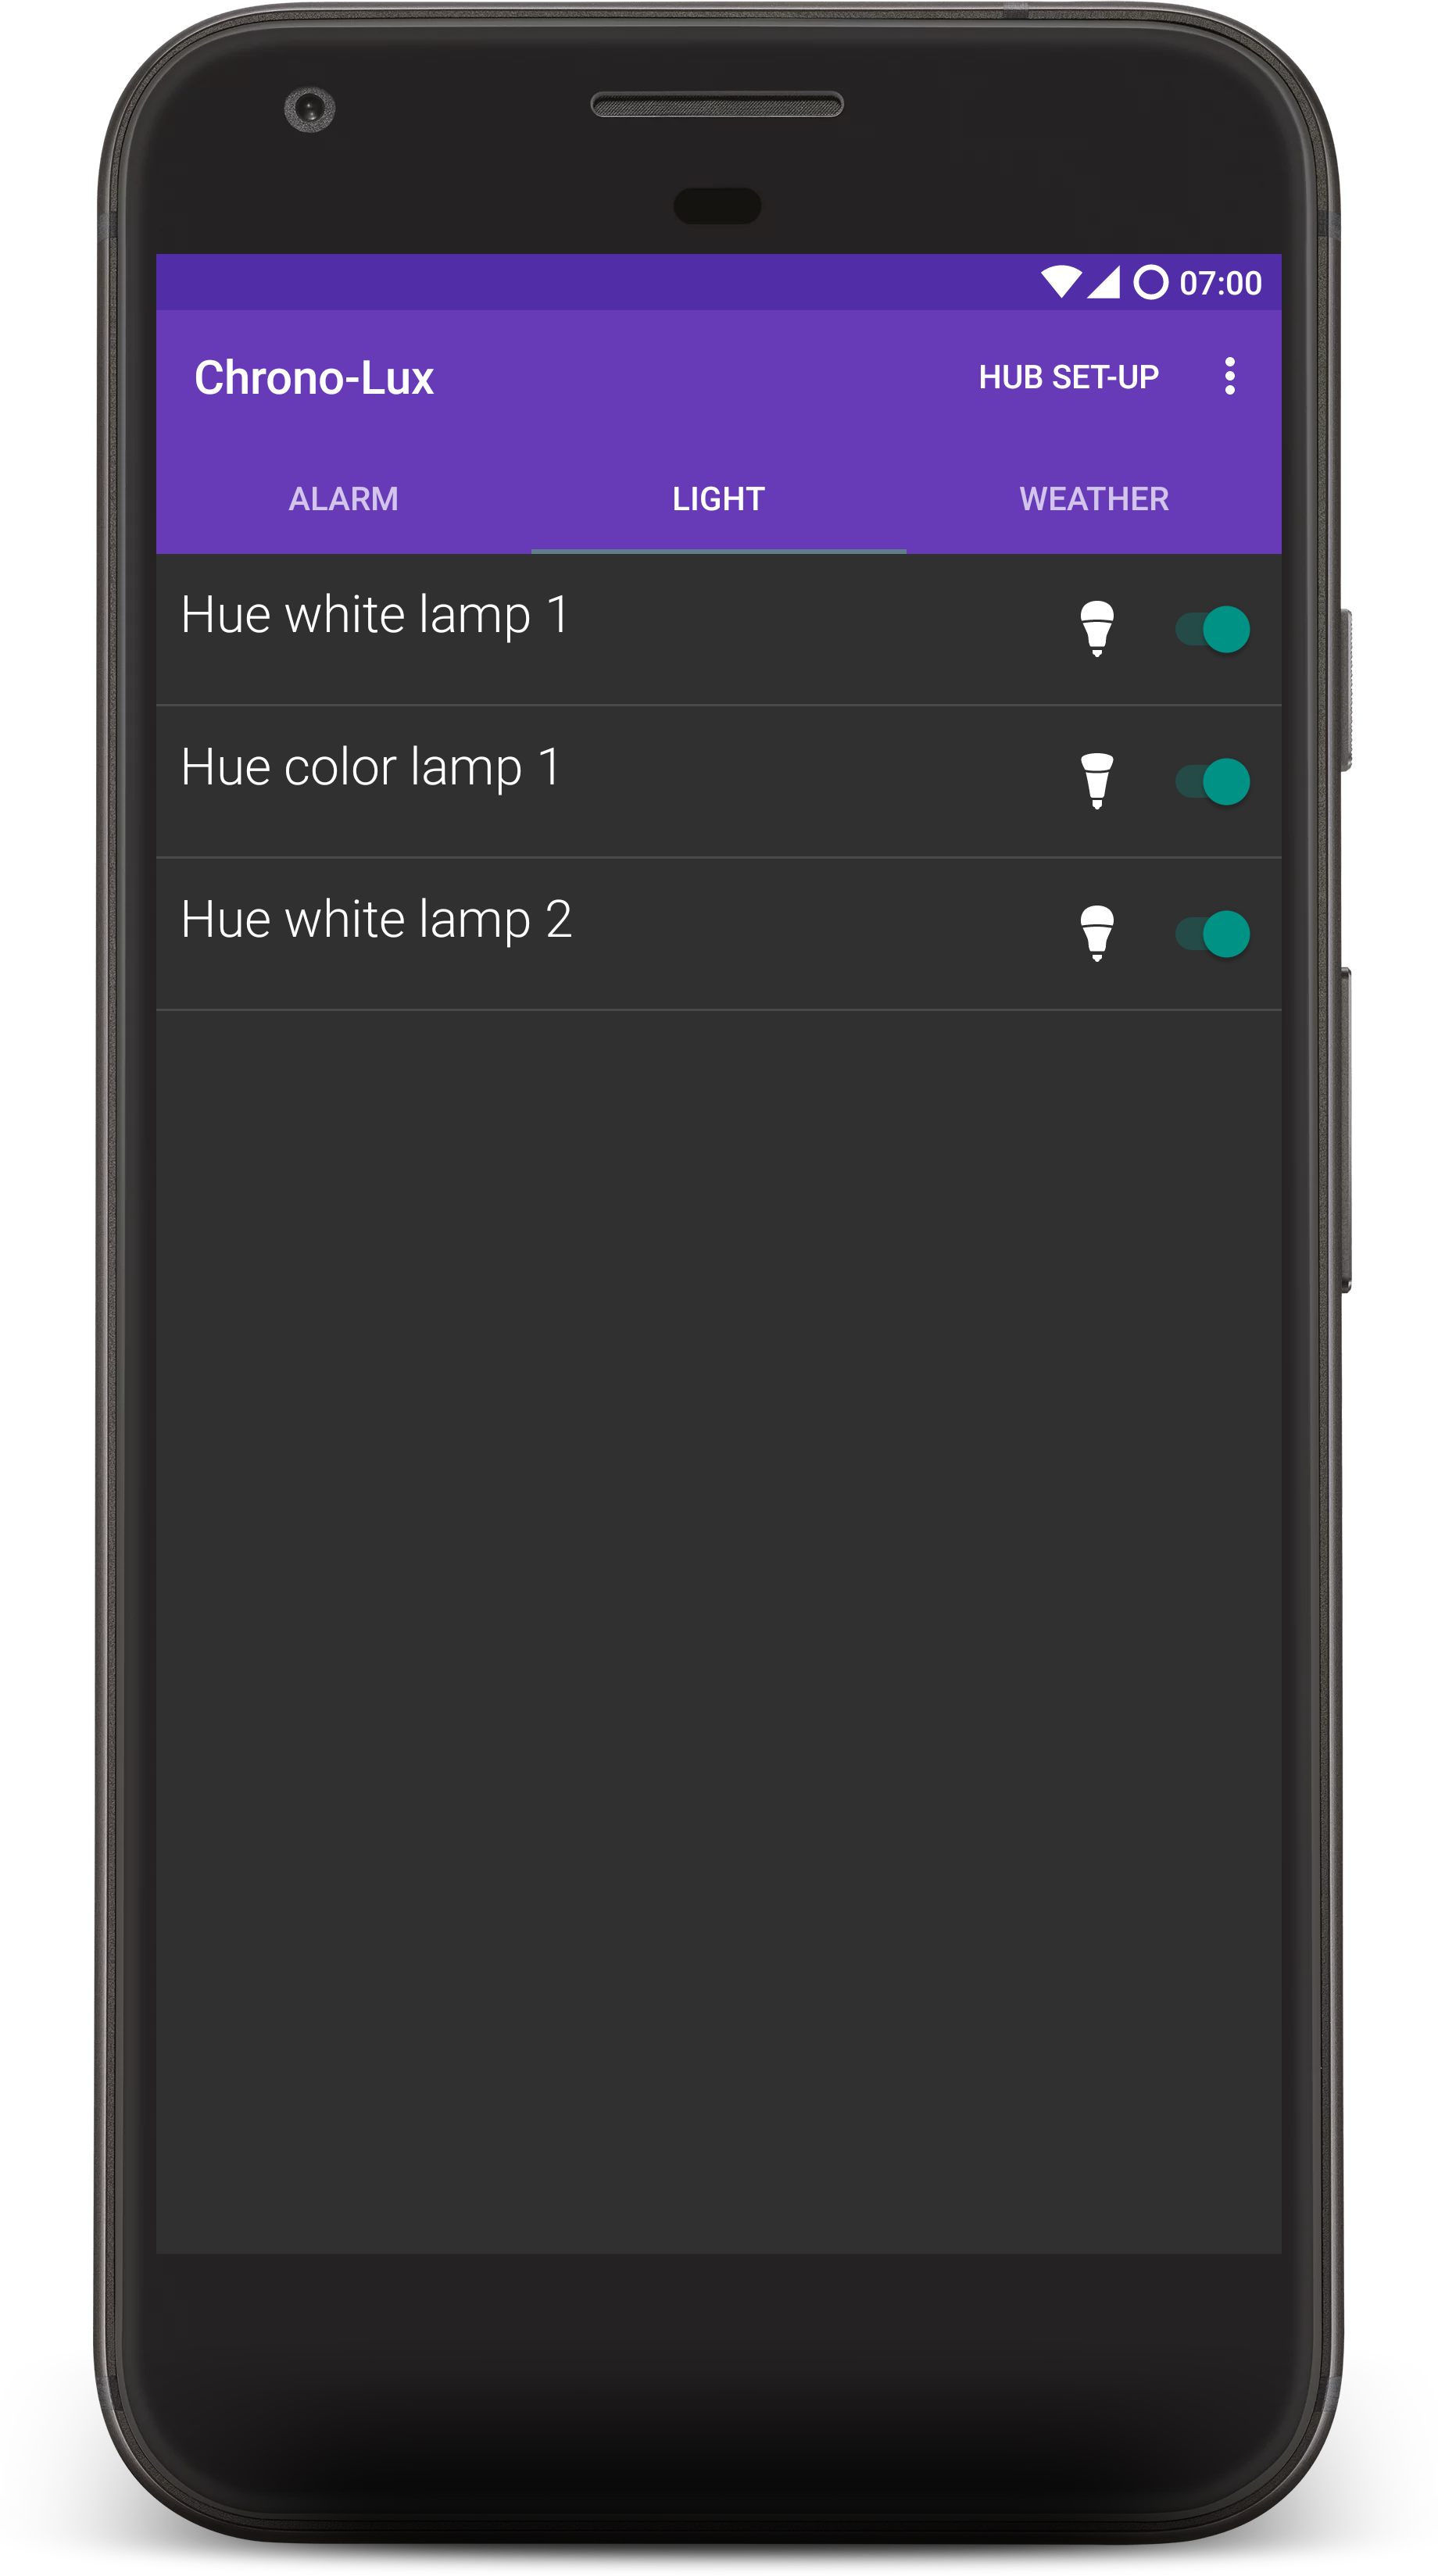
\includegraphics[scale=0.1]{Images/lightList.png}
  \caption{List of available lights}
  \label{fig:lightList}
\end{figure}

\subsubsection{Toggling the lights}\label{toggling-the-lights}

Any lights assigned to the bridge will be displayed in a list,
displaying their name and an icon indicating the light type.

Each alarm can be turned on/off easily by tapping the switch on the
right hand side of the screen.

It should be noted that if a light is turned off at the wall/switch the
last known light state will be displayed within the application when
displayed.

\subsection{Weather}\label{weather}

Weather will be displayed on the weather tab. To change the location of
the weather being displayed, press on the menu expansion button from
anywhere within the application as seen in figure \ref{fig:setcity},
this will display the option to change the city stored.

\begin{figure}[H]
  \centering
  \subfloat[The options menu is in the top right]{{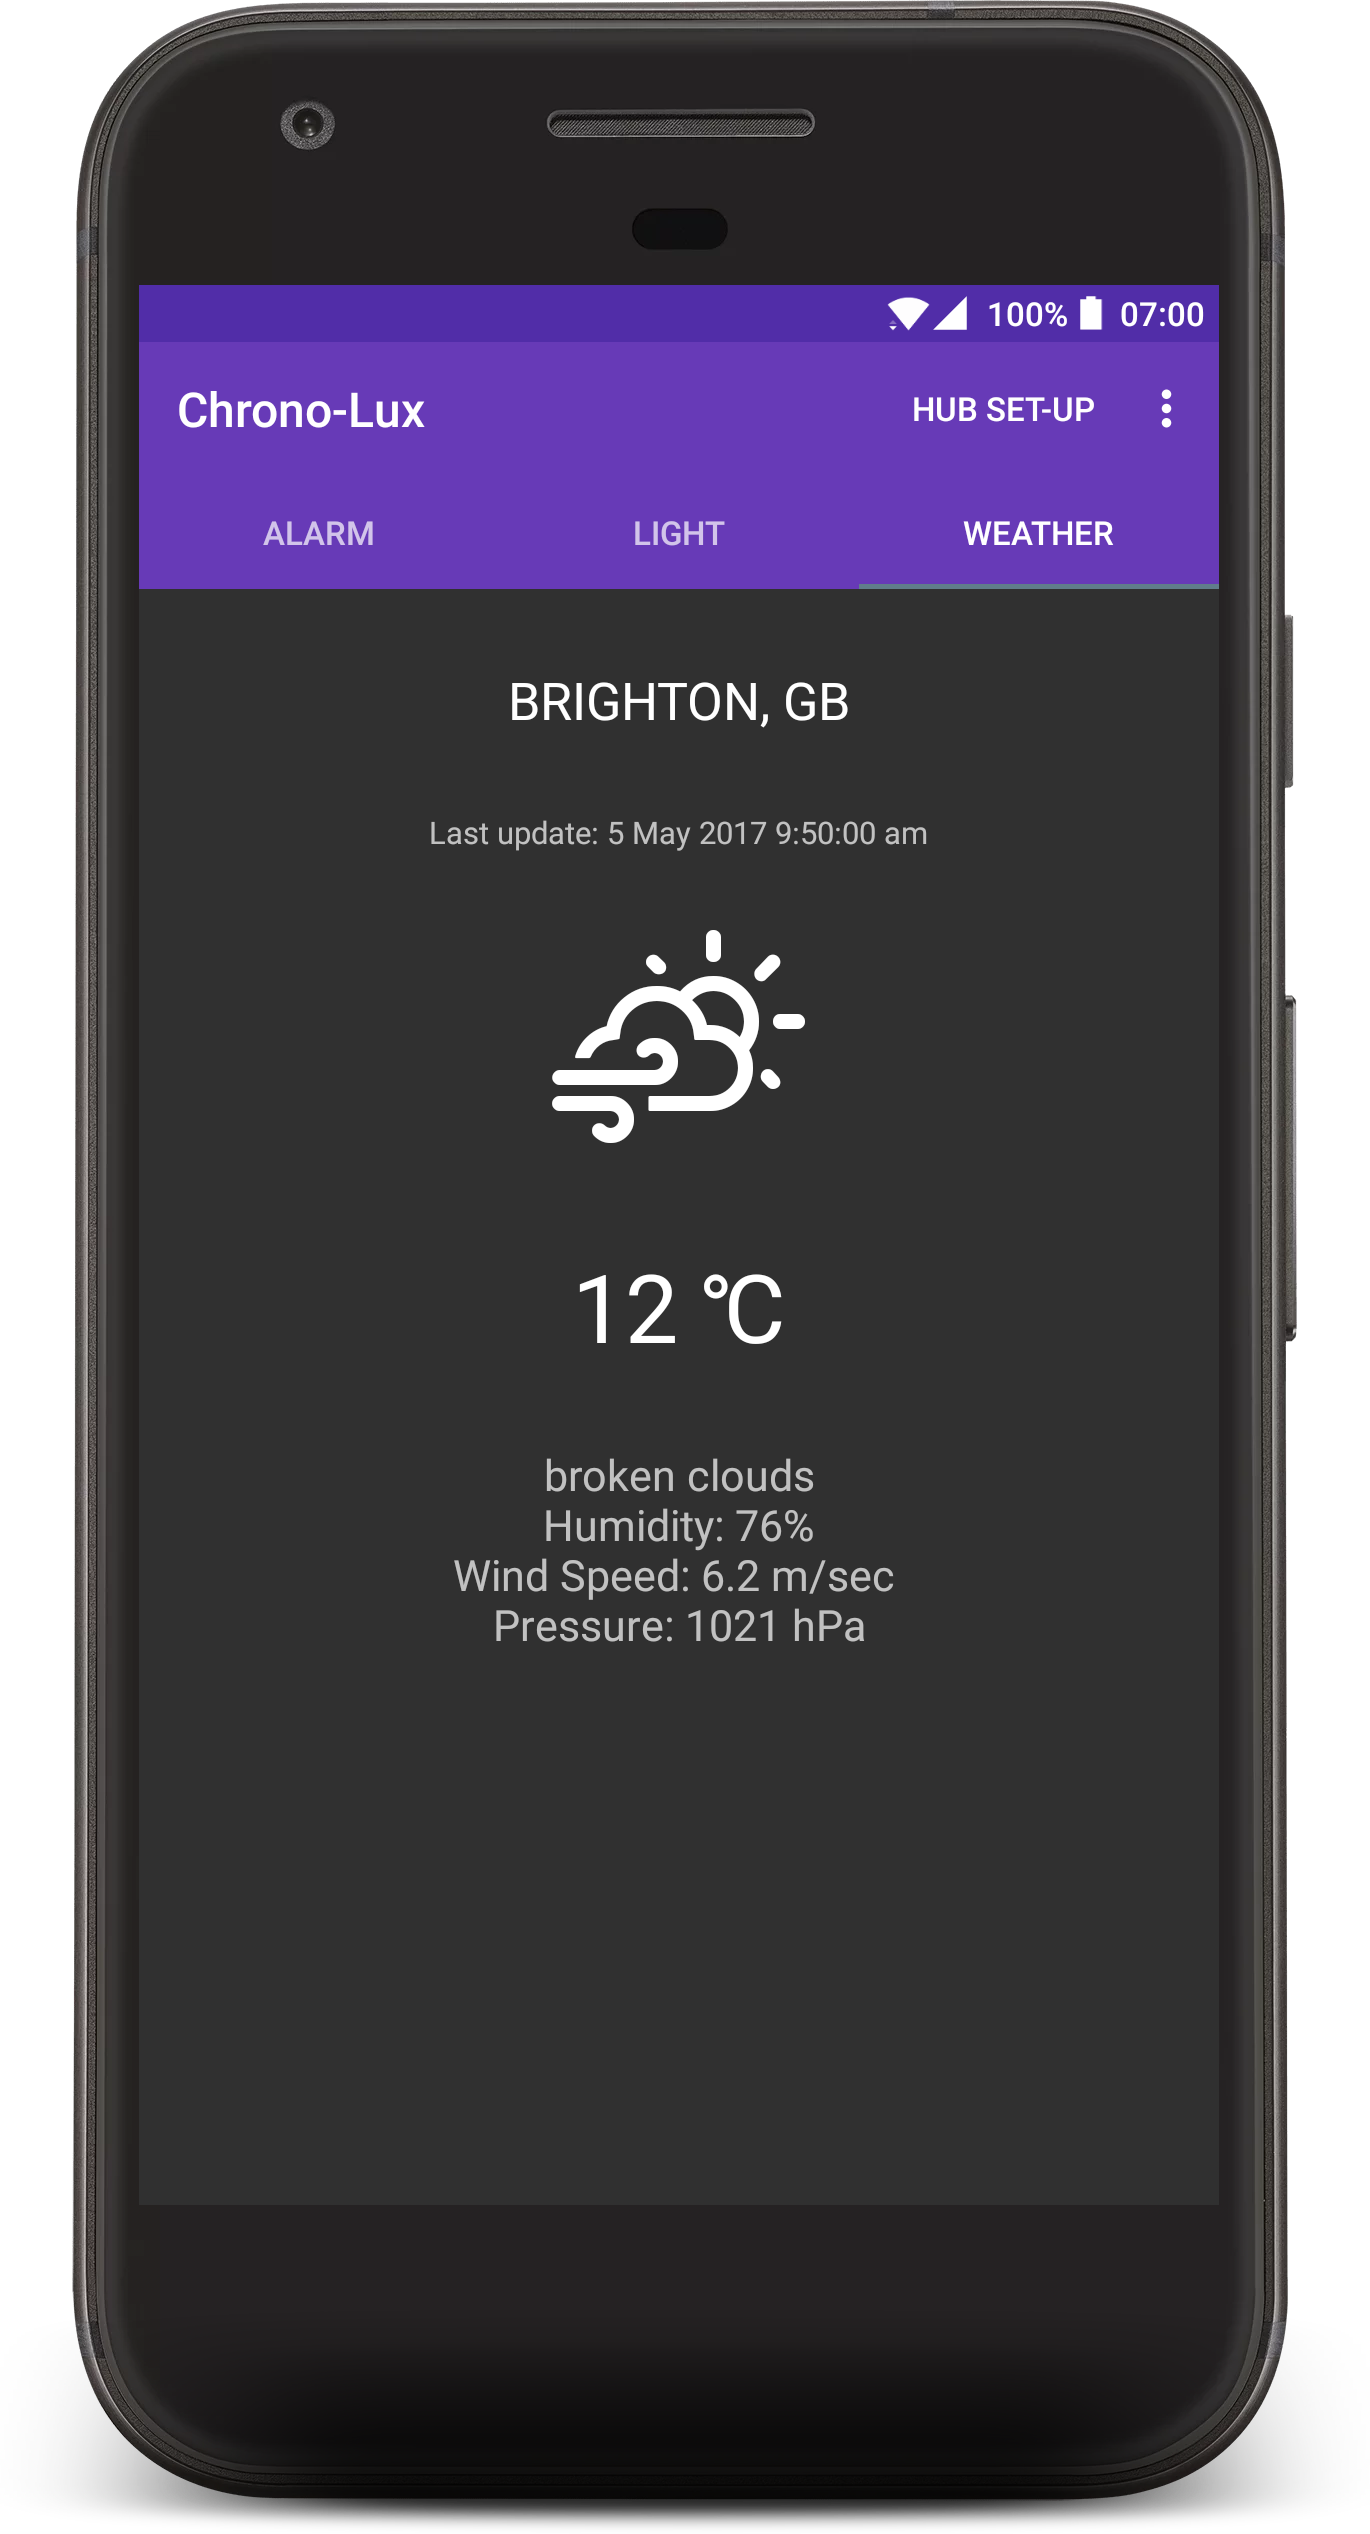
\includegraphics[scale=0.1]{./Images/optionmenu.png}}}
  \qquad
  \subfloat[Change city option]{{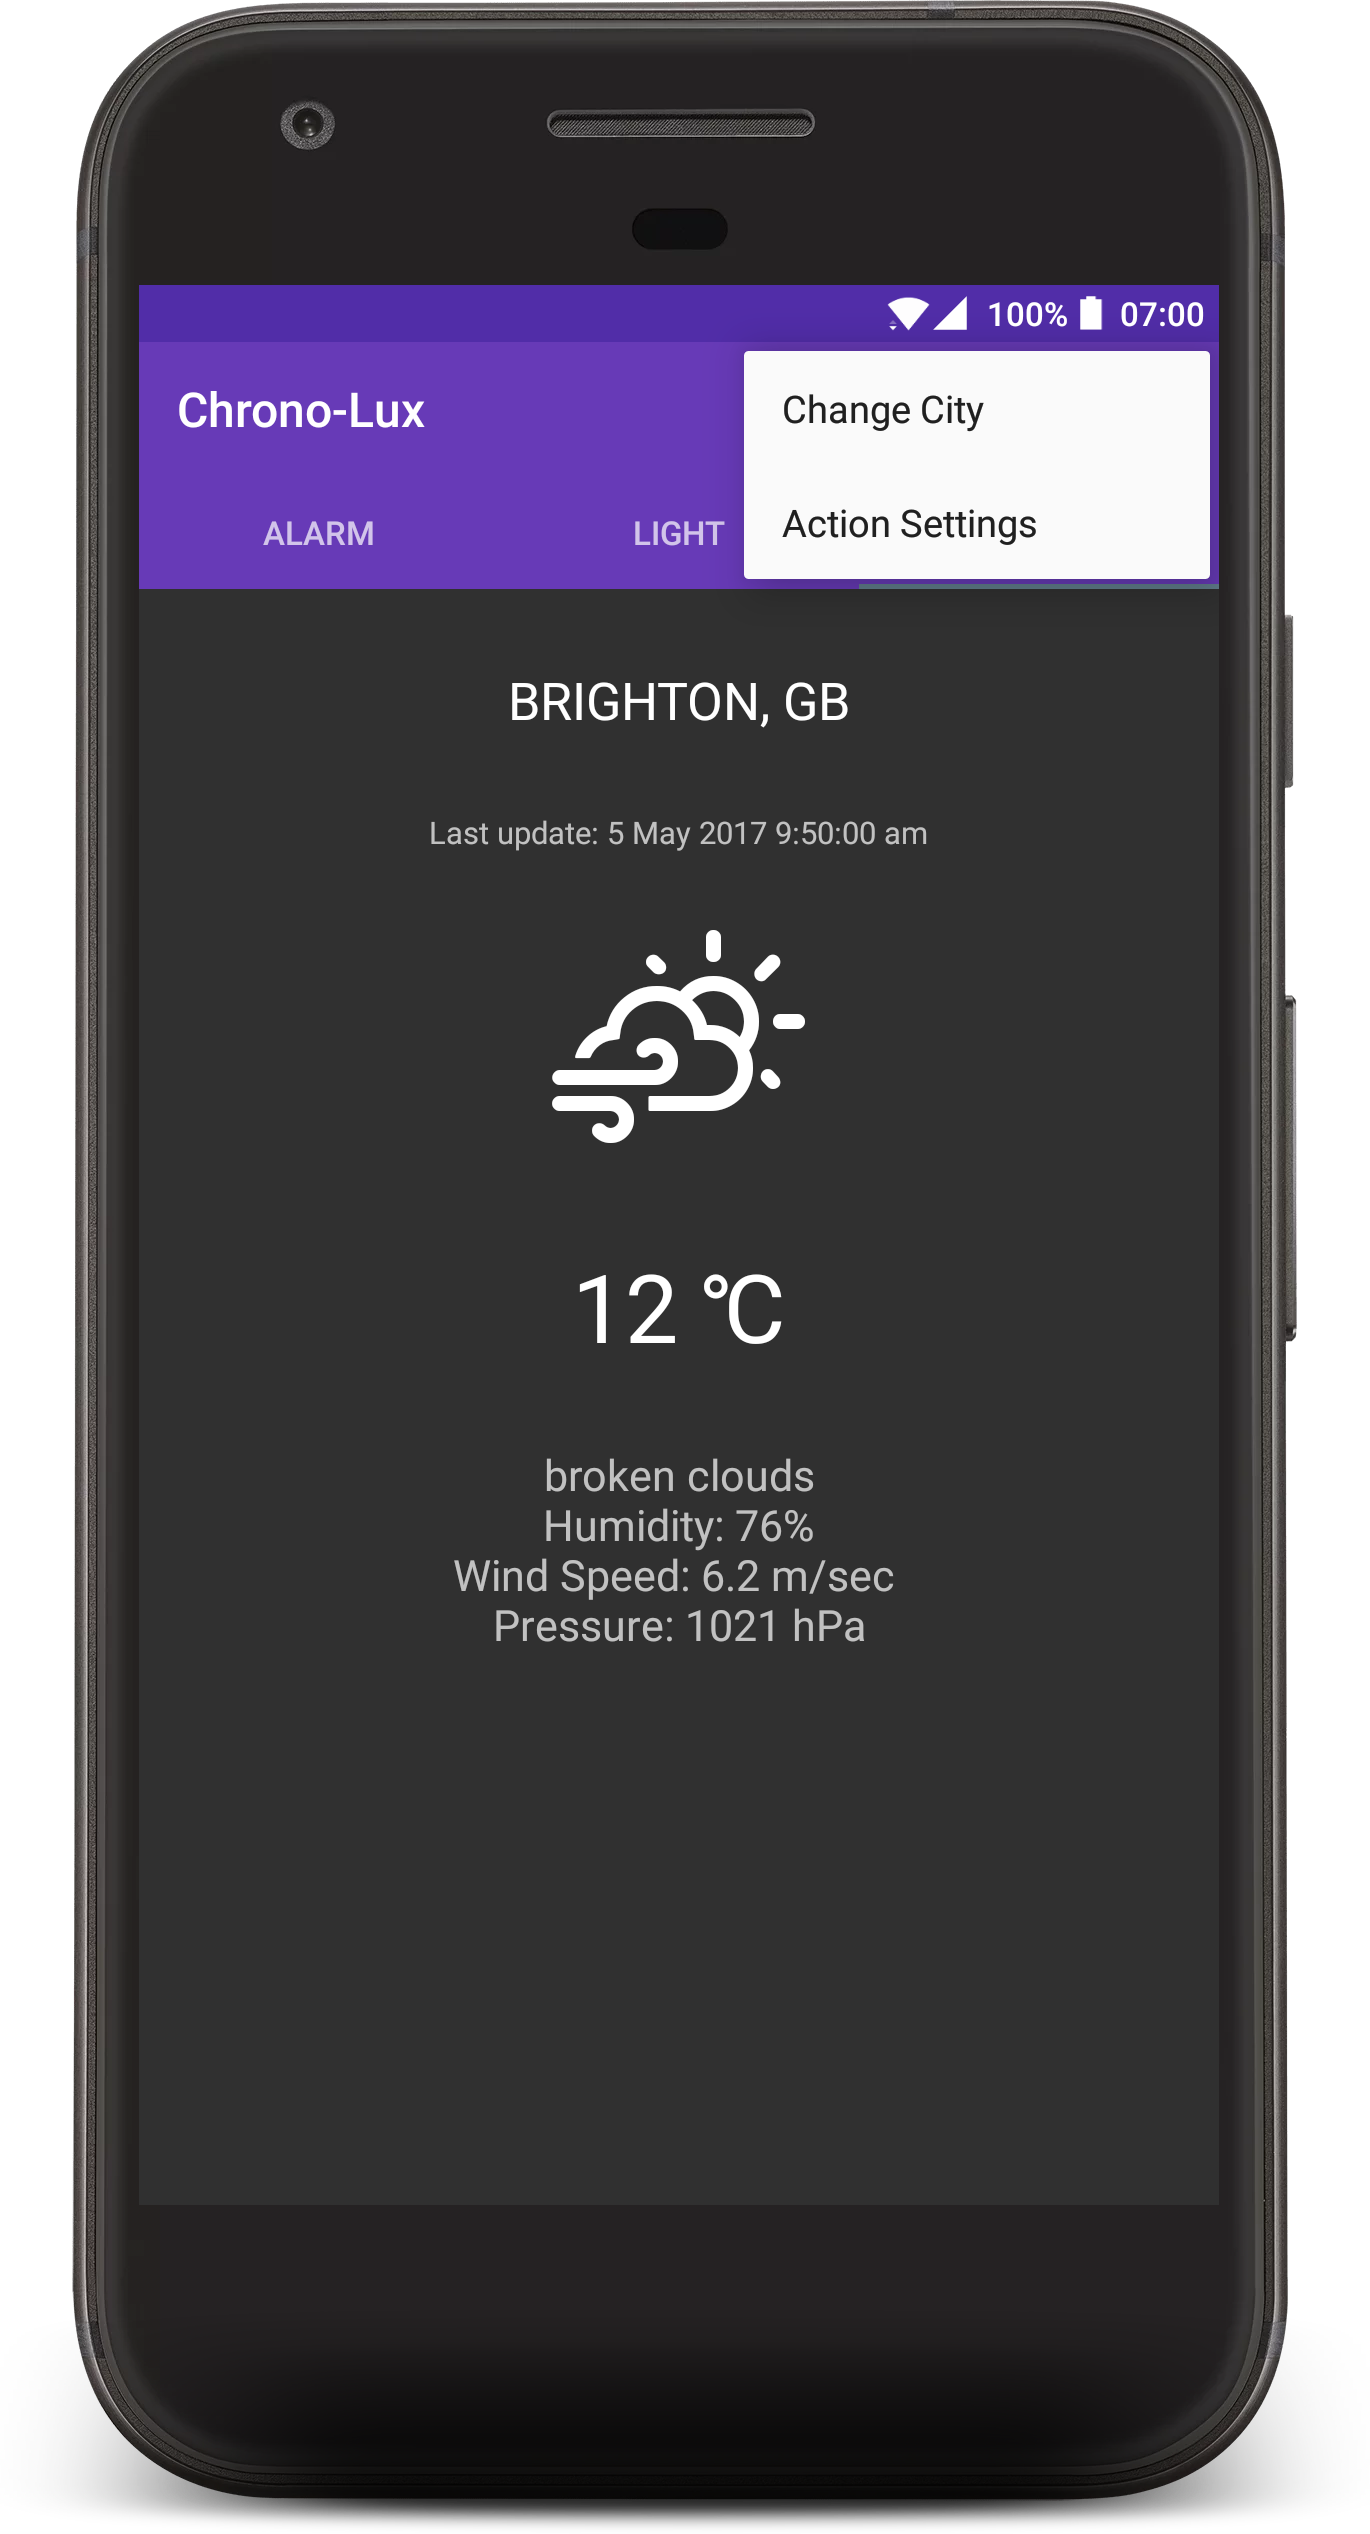
\includegraphics[scale=0.1]{./Images/changecityoption.png}}}
  \caption{The city selection option}%
  \label{fig:setcity}%
\end{figure}

when the change city option is selected a text dialog will appear
allowing for the entry of a different city, simply type in the name of
the city desired and accept the change, the weather will be updated when
the weather tab is loaded next.


\end{document}
